\documentclass{elektr}
\usepackage{hyperref}
\hypersetup{colorlinks=true,urlcolor=blue,citecolor=blue}
\usepackage[all]{xy,xypic}
\usepackage{amsfonts,amssymb,amsmath,amsgen,amsopn,amsbsy,theorem,graphicx,epsfig}
\usepackage{amscd,bezier,latexsym,mathrsfs,eurosym,enumerate}
\usepackage[utf8]{inputenc}
\usepackage[english]{babel}
\usepackage{cleveref,multirow}
\usepackage[dvipsnames,table]{xcolor}
\usepackage[pagewise]{lineno}
\usepackage{enumitem}
\usepackage[most]{tcolorbox}
\usepackage[colorinlistoftodos,prependcaption,textsize=tiny]{todonotes}
\usepackage[numbers,sort&compress]{natbib}

\usepackage{linguex}
\usepackage{stmaryrd}
\usepackage{leipzig}
\makeglossaries
\newleipzig{Der}{Der}{Derivation}
\newleipzig{Ant}{Ant}{Anterior}
\usepackage{tikz-dependency}
\usepackage{multicol}

\yil{}
\vol{}
\fpage{}
\lpage{}
\doi{}

\title{A collaborative grammatical annotation tool for agglutinative languages}

\author[]{
\textbf{}\\

\rec{.202}
\acc{.202}
\finv{..202}
}

% \def\E{\ifmmode{\mathbb E}\else{$\mathbb E$}\fi} %natural numbers
\def\N{\ifmmode{\mathbb N}\else{$\mathbb N$}\fi} %natural numbers
\def\R{\ifmmode{\mathbb R}\else{$\mathbb R$}\fi} %real numbers
\def\Q{\ifmmode{\mathbb Q}\else{$\mathbb Q$}\fi} %rational numbers
\def\C{\ifmmode{\mathbb C}\else{$\mathbb C$}\fi} %complex numbers
\def\H{\ifmmode{\mathbb H}\else{$\mathbb H$}\fi} %complex numbers
\def\Z{\ifmmode{\mathbb Z}\else{$\mathbb Z$}\fi} %integers
\def\P{\ifmmode{\mathbb P}\else{$\mathbb P$}\fi} %real numbers
\def\T{\ifmmode{\mathbb T}\else{$\mathbb T$}\fi} %real numbers
\def\SS{\ifmmode{\mathbb S}\else{$\mathbb S$}\fi} %real numbers
\def\DD{\ifmmode{\mathbb D}\else{$\mathbb D$}\fi} %real numbers

\renewcommand{\a}{\alpha}
\renewcommand{\b}{\beta}
\renewcommand{\d}{\delta}
\newcommand{\D}{\Delta}
%\newcommand{\e}{\epsilon}
\newcommand{\var}{\varepsilon}
\newcommand{\g}{\gamma}
\newcommand{\la}{\lambda}
\newcommand{\La}{\Lambda}
\newcommand{\lan}{\langle}
\newcommand{\ran}{\rangle}
\newcommand{\n}{\nabla}
\newcommand{\va}{\varphi}
\newcommand{\s}{\sigma}
\newcommand{\Sig}{\Sigma}
\renewcommand{\t}{\tau}
\renewcommand{\th}{\theta}
\newcommand{\Om}{\Omega}
\newcommand{\om}{\omega}
\newcommand{\pa}{\partial}
\newcommand{\up}{\upsilon}
\newcommand{\vp}{\varphi}
%\newcommand{\z}{\zeta}





\newcommand{\bse}{\begin{subequations}}
\newcommand{\ese}{\end{subequations}}
\newcommand{\ben}{\begin{enumerate}}
\newcommand{\een}{\end{enumerate}}
\newcommand{\bens}{\begin{enumerate*}}
\newcommand{\eens}{\end{enumerate*}}
\newcommand{\be}{\begin{equation}}
\newcommand{\ee}{\end{equation}}
\newcommand{\bea}{\begin{eqnarray}}
\newcommand{\eea}{\end{eqnarray}}
\newcommand{\baa}{\begin{eqnarray*}}
\newcommand{\eaa}{\end{eqnarray*}}
\newcommand{\bc}{\begin{center}}
\newcommand{\ec}{\end{center}}
\newcommand{\ol}{\overline}
\newcommand{\ul}{\underline}
\newcommand{\ov}{\overbrace}
\newcommand{\uv}{\underbrace}
\newcommand{\Ra}{\Rightarrow}
\newcommand{\ra}{\rightarrow}
\newcommand{\ds}{\displaystyle}
\newcommand{\vs}{\vspace}


\newcommand{\IR}{\mbox{I \hspace{-0.2cm}R}}
\newcommand{\IN}{\mbox{I \hspace{-0.2cm}N}}



%% \theoremstyle{plain} %% This is the default

\newtheorem{theorem}{Theorem}%[section]

% \theoremstyle{corollary}
\newtheorem{corollary}{Corollary}

% \theoremstyle{lemma}
\newtheorem{lemma}{Lemma}

% \theoremstyle{proposition}
\newtheorem{proposition}{Proposition}

% \theoremstyle{axiom}
\newtheorem{axiom}{Axiom}

% \theoremstyle{conjecture}
\newtheorem{conjecture}{Conjecture}

% \theoremstyle{example}
\newtheorem{example}{Example}

% \theoremstyle{definition}
\newtheorem{definition}{Definition}%[section]

% \theoremstyle{remark}
\newtheorem{remark}{Remark}%[section]
\newtheorem{notation}{Notation}


\newtheorem{question}{Question}%[section]
\newtheorem{construction}{Construction}

\newtheorem{athm}{Theorem}
\renewcommand{\theathm}{\Alph{athm}}



\def\E{\ifmmode{\mathbb E}\else{$\mathbb E$}\fi} %natural numbers
\def\N{\ifmmode{\mathbb N}\else{$\mathbb N$}\fi} %natural numbers
\def\R{\ifmmode{\mathbb R}\else{$\mathbb R$}\fi} %real numbers
\def\Q{\ifmmode{\mathbb Q}\else{$\mathbb Q$}\fi} %rational numbers
\def\C{\ifmmode{\mathbb C}\else{$\mathbb C$}\fi} %complex numbers
\def\H{\ifmmode{\mathbb H}\else{$\mathbb H$}\fi} %complex numbers
\def\Z{\ifmmode{\mathbb Z}\else{$\mathbb Z$}\fi} %integers
\def\P{\ifmmode{\mathbb P}\else{$\mathbb P$}\fi} %real numbers
\def\T{\ifmmode{\mathbb T}\else{$\mathbb T$}\fi} %real numbers
\def\SS{\ifmmode{\mathbb S}\else{$\mathbb S$}\fi} %real numbers
\def\DD{\ifmmode{\mathbb D}\else{$\mathbb D$}\fi} %real numbers

\renewcommand{\a}{\alpha}
\renewcommand{\b}{\beta}
\renewcommand{\d}{\delta}
\newcommand{\D}{\Delta}
%\newcommand{\e}{\epsilon}
\newcommand{\var}{\varepsilon}
\newcommand{\g}{\gamma}
\newcommand{\la}{\lambda}
\newcommand{\La}{\Lambda}
\newcommand{\lan}{\langle}
\newcommand{\ran}{\rangle}
\newcommand{\n}{\nabla}
\newcommand{\va}{\varphi}
\newcommand{\s}{\sigma}
\newcommand{\Sig}{\Sigma}
\renewcommand{\t}{\tau}
\renewcommand{\th}{\theta}
\newcommand{\Om}{\Omega}
\newcommand{\om}{\omega}
\newcommand{\pa}{\partial}
\newcommand{\up}{\upsilon}
\newcommand{\vp}{\varphi}
%\newcommand{\z}{\zeta}





\newcommand{\bse}{\begin{subequations}}
\newcommand{\ese}{\end{subequations}}
\newcommand{\ben}{\begin{enumerate}}
\newcommand{\een}{\end{enumerate}}
\newcommand{\bens}{\begin{enumerate*}}
\newcommand{\eens}{\end{enumerate*}}
\newcommand{\be}{\begin{equation}}
\newcommand{\ee}{\end{equation}}
\newcommand{\bea}{\begin{eqnarray}}
\newcommand{\eea}{\end{eqnarray}}
\newcommand{\baa}{\begin{eqnarray*}}
\newcommand{\eaa}{\end{eqnarray*}}
\newcommand{\bc}{\begin{center}}
\newcommand{\ec}{\end{center}}
\newcommand{\ol}{\overline}
\newcommand{\ul}{\underline}
\newcommand{\ov}{\overbrace}
\newcommand{\uv}{\underbrace}
\newcommand{\Ra}{\Rightarrow}
\newcommand{\ra}{\rightarrow}
\newcommand{\ds}{\displaystyle}
\newcommand{\vs}{\vspace}


\newcommand{\IR}{\mbox{I \hspace{-0.2cm}R}}
\newcommand{\IN}{\mbox{I \hspace{-0.2cm}N}}



%% \theoremstyle{plain} %% This is the default

\newtheorem{theorem}{Theorem}%[section]

% \theoremstyle{corollary}
\newtheorem{corollary}{Corollary}

% \theoremstyle{lemma}
\newtheorem{lemma}{Lemma}

% \theoremstyle{proposition}
\newtheorem{proposition}{Proposition}

% \theoremstyle{axiom}
\newtheorem{axiom}{Axiom}

% \theoremstyle{conjecture}
\newtheorem{conjecture}{Conjecture}

% \theoremstyle{example}
\newtheorem{example}{Example}

% \theoremstyle{definition}
\newtheorem{definition}{Definition}%[section]

% \theoremstyle{remark}
\newtheorem{remark}{Remark}%[section]
\newtheorem{notation}{Notation}


\newtheorem{question}{Question}%[section]
\newtheorem{construction}{Construction}

\newtheorem{athm}{Theorem}
\renewcommand{\theathm}{\Alph{athm}}

% \newcommand{\conllu}{\textsc{c}o\textsc{nll-u}}
\newcommand{\boatvone}{\textsc{b}o\textsc{at}-{\scriptsize v1}}
\newcommand{\boatvtwo}{\textsc{b}o\textsc{at}-{\scriptsize v2}}
\newcommand{\bountreebank}{\textsc{boun} Treebank}

\newcommand{\upos}{\textsc{upos}}
\newcommand{\propn}{\textsc{propn}}
\newcommand{\head}{\textsc{head}}
\newcommand{\deprel}{\textsc{deprel}}
\newcommand{\form}{\textsc{form}}
\newcommand{\lemma}{\textsc{lemma}}
\newcommand{\feats}{\textsc{feats}}
\newcommand{\noun}{\textsc{noun}}

\newcommand{\ud}{\textsc{ud}}


\newcommand{\conllu}{\textsc{c}o\textsc{nll-u}}
\newcommand{\conll}{\textsc{c}o\textsc{nll}}
\newcommand{\boat}{\textsc{b}o\textsc{at}}
\newcommand{\boatvone}{\textsc{b}o\textsc{at}-{\scriptsize v1}}
\newcommand{\boatvtwo}{\textsc{b}o\textsc{at}-{\scriptsize v2}}
\newcommand{\bountreebank}{\textsc{boun} \textsc{T}reebank}

\newcommand{\propn}{\textsc{propn}}
\newcommand{\id}{\textsc{id}}
\newcommand{\form}{\textsc{form}}
\newcommand{\udlemma}{\textsc{lemma}}
\newcommand{\upos}{\textsc{upos}}
\newcommand{\xpos}{\textsc{xpos}}
\newcommand{\feats}{\textsc{feats}}
\newcommand{\head}{\textsc{head}}
\newcommand{\deprel}{\textsc{deprel}}
\newcommand{\deps}{\textsc{deps}}
\newcommand{\misc}{\textsc{misc}}
\newcommand{\noun}{\textsc{noun}}

\newcommand{\ud}{\textsc{ud}}

\setcounter{page}{1}
\begin{document}

\maketitle

% \begin{abstract}
The value of quality treebanks is steadily increasing due to the important role they play in the development of natural language processing tools.
The creation of such treebanks is enormously labour-intensive and time consuming.
Therefore, tools that support the annotation process are very valuable.
This is especially the case for morphologically rich languages.
The \boat{} annotation tool was developed for annotating dependency relations, which was used to create the manually annotated \bountreebank{} (UD\_Turkish-BOUN) of Turkish National Corpus (TNC).
The extensive annotation experience revealed several opportunities of improvement.
Combined with our desire to create a multi-user web based annotation tool, this led to the development of \boat{} v2.
The main objectives of the new tool are to: (1) provide further support for creating valid and consistent annotations, (2) significantly improve the user experience of the annotator, and (3) develop an open source and easily deployable web-based annotation tool and an API to benefit the scientific and education community.
This paper discusses the requirements, design, implementation of \boat{} v2 with annotation examples that highlight the new features.
\end{abstract}

\begin{abstract}
The significance of high-quality treebanks has been steadily increasing due to their crucial role in developing natural language processing tools.
The creation of such treebanks is an enormously labor-intensive and time-consuming task due to the need for qualified annotators and the quantity of data to be annotated.
Tools that facilitate the annotation process have been developed, however, their interfaces are usually designed for analytic languages.
Agglutinative languages tend to be richer in their morphology and require extensive annotations that significantly differ from annotations in analytic languages.
Most of these tools are not well-suited for annotations in agglutinative languages such as Turkish.
As such, low-resource agglutinative languages need suitable tools to accelerate the creation of high-quality data resources.
This paper describes the design and implementation of a web-based collaborative grammatical annotation tool designed to expedite and facilitate the annotation of large treebanks, especially in agglutinative languages.
This work builds on extensive experience with another grammatical annotation tool developed previously to annotate a Turkish treebank.
The main objectives of this tool are to: (1) support the creation of valid and consistent annotations, (2) increase the speed of the annotation process, (3) improve the user experience of annotators, (4) support collaboration among annotators, and (5) provide an easily deployable and open-source web-based annotation tool with an application programming interface (API) to benefit the scientific community.
This paper discusses the requirements elicitation, design, implementation, and evaluation of this tool along with examples.

\keywords{Natural language processing, Linguistic annotation, Annotation tool, Web application, Dependency parsing, Universal dependencies}

\end{abstract}    

% \section{Introduction}
\label{sec:introduction}

Treebanks are important resources in the development of natural language processing tools.
Quality tools need treebanks that are manually annotated by linguistic experts. 
This is especially true for agglutinative languages due to their complex morphologies. 
The creation of such treebanks is highly labor-intensive and time-consuming due to the meticulous attention required.
Thus, tools that support this process are very important.

% may need a better segue
In recent years, there have been significant efforts to bridge the gap in data resources available for agglutinative low-resource languages.
%Among them is the creation of quality annotated data resources.
Unfortunately, annotation tools developed for analytical languages~\cite{UD} are not to be well suited for agglutinative languages with their complex morphology.
The annotation of agglutinative  languages requires significantly more operations, such as entering several features for each lemma and sometimes even for split lemmas.
Annotation tools that rely on drag-drop and mouse-based interfaces, which seem appealing, are not suitable when entering numerous features is necessary since swapping between input modalities disrupts the flow of concentration.

\boatvone~\cite{turk2021resources} is an annotation tool that was developed to support the dependency annotation of MRLs to produce treebanks compliant with the Universal Dependency framework~\cite{UD}.
It is a standalone application developed using Python and Qt for the user interface.
Its main input modality is via the keyboard on request of the annotators. 
It was used to create the \bountreebank~\cite{turk-etal-2019-turkish,turk2021resources,UD-Boun-Treebank} -- a manually annotated Turkish dependency treebank comprising of thousands of sentences.
This experience revealed several points of improvement for such annotation tools.
% Note: logically doesn't flow after previous statmement. Also, efficiency of a keyboard-oriented approach over an approach of switching between mouse and keyboard was validated in the aforementioned annotation work.
The main takeaway was a much better understanding of the time, effort, cognitive load, and extra information requirements of the annotation process.
Improvements regarding these aspects should, consequently, produce higher quality data resources.

This work presents a dependency annotation tool (\boatvtwo) that has been designed based on the experience with \boatvone.
The design and implementation of the tool aimed to: (1) support the creating valid and consistent annotations with increased speed, (2) significantly improve the user experience of the annotator, (3) allow collaboration among annotators during the annotation process, and (4) provide an open source and easily deployable web-based annotation tool with an API to benefit the scientific community.
The development started with requirements elicitation, for which earlier experiences and in-depth interviews with an experienced annotator were taken into account.

\boatvtwo\ is a web-based collaborative dependency annotation tool that focuses on the user experience of annotators. 
It has and application programming interface (API) for programmatic access and extensibility. 
The tool is dockerized in to facilitate accessibility and ease of  deployment.
The current prototype is being evaluated with positive feedback.
The final version will be made available on the Boğaziçi University's NLP platform~\cite{DIP} and provided as an open source resource.
% This is better in Requirement section. This feedback indicated that the ability to collaborate within the tool is needed to increase efficiency of multi-annotator treebank creation.
% Requirements In light of the feedback, we developed a web application that supports multiple users to enable a collaborative environment for annotations.
% An API was designed to render the functionalities accessible to various NLP applications.
%Several user experience improvements were implemented in order to facilitate the flow of an annotation session.
The main contributions of this work are:
\begin{itemize}
\setlength\itemsep{0em}
        \item Design of a dependency annotation tool that is based on requirements elicited from experienced annotators who are linguists,
        \item The development of a tool that takes into account the annotator experience to improve resulting annotations,
        \item Support for multi-users to provide indivual spaces for annotations, computation of inter-annotator agreements, and other potential collaboration,
        \item The development of a web-based annotation tool based on a supporting API, and
        \item Packaging of the tool to support easy access by virtualizing it using Docker and providing the code as an open source resource.
\end{itemize}

The remainder of this paper is organized as follows:
Section~\ref{sec:related} presents related work,
Section~\ref{sec:requirements} describes the requirements elicitation process and design,
Section~\ref{sec:implementation} presents the implementation with emphasis on the new features,
Section~\ref{sec:annotation} presents a use case of annotation.
We discuss our experiences and point out some future work in Section~\ref{sec:discussion} and offer our conclusions  in Section~\ref{sec:conclusion}.

\section{Introduction}
\label{sec:introduction}

Treebanks are significant resources in the development of natural language processing (NLP) tools and resources, and quality NLP resources need quality treebanks, manually annotated by linguistic experts.
This is particularly true for agglutinative languages due to their complex morphologies.
The creation of quality treebanks in morphologically rich languages (MRL) is highly labor-intensive and time-consuming due to the sheer amount of meticulous attention and effort required.
Thus, annotation tools that support this process are essential.
In recent years, there have been major efforts in increasing the data resources available for low-resource agglutinative languages --such as introducing new datasets and re-annotating existing treebanks.
All these efforts require grammatical annotation by native speakers and/or linguistic experts.

Grammatical annotation involves marking each token of a sentence with corresponding linguistic values.
Universal Dependencies~\cite{ud} (\ud) is one of the most widely accepted frameworks for morphosyntactic grammar annotations as it offers the flexibility and coherency needed to cover typologically very different languages in a unified way.
The annotation format of \ud\ called \conllu~\cite{conll} (Computational Natural Language Learning) defines a set of linguistic tags to express syntactic category (e.g. noun, verb, adjective) and morphological features of each token as well as the relationship between them.
The \conllu\ format has 10 columns for each token of a sentence where the annotator can mark down word form, lemma form, syntactic category, dependency relation, and more, following predetermined rules and tags.
For example, the universal part of speech (\upos) column is used to denote the syntactic category of a token while the features (\feats) column allows marking morphosyntactic features such as case, number, or tense.
Since agglutinative languages allow stacking multiple morphemes on roots and stems for inflection, the \feats\ column is heavily used in their annotations to mark several values for each token.
This makes the effort required to annotate agglutinative languages significantly higher than analytic languages.
Annotation tools with drag-drop and mouse-based interfaces, although appealing, are not well suited for agglutinative languages as they require alternating among input modalities frequently, disrupting the flow and slowing down the annotator.

Aware of this issue, \boatvone~\cite{anon} was developed to support the annotation of morphologically rich languages to produce treebanks compliant with the \ud\ framework~\cite{ud}.
\boatvone\ allowed annotations via using only the keyboard, yet the user experience revealed several points of improvement.
The main takeaway from the feedback provided by the annotators that had used \boatvone\ was a much better understanding of the time, effort, cognitive load, and extra information requirements of the annotation process.
Improvements regarding these aspects should improve the performance of annotators, and consequently, produce higher-quality NLP resources.

This work presents a web-based collaborative grammatical annotation tool (\boatvtwo) that has been designed based on earlier experiences and requirement elicitation sessions with experienced annotators~\footnote{An earlier version of this paper was presented at the The International Conference on Agglutinative Language Technologies as a challenge of Natural Language Processing (ALTNLP)~\cite{anon} in 2022.}.
In light of the feedback from this experience, several user experience improvements were implemented to enhance the flow and consistency of the annotators.
Additionally, this tool was designed as a web application that supports multiple users to enable a collaborative environment for annotators.
The design and implementation of the tool aimed to: (1) support the creation of valid and consistent annotations, (2) increase the speed of the annotation process, (3) improve the user experience of annotators, (4) support collaboration among annotators, and (5) provide an open-source and easily deployable web-based annotation tool with an API to benefit the scientific community.
The development started with requirements elicitation, for which earlier experiences and in-depth interviews with an experienced annotator were taken into account.
The main issues identified during the requirement analysis phase are:
\begin{itemize}
\setlength\itemsep{0em}
\item The interface must be free of clutter and intuitive so that the annotator can focus on the task better.
\item New features like auto-completion should be introduced to increase the speed of the annotator.
\item Problems detected after extensive use of \boatvone\ must be addressed.
\item Support for collaboration has become significant since the increase in the effort to annotate large treebanks has led to the need for multiple annotators.
\end{itemize}

Considering the key points above, \boatvtwo\ was designed in line with the typological particularities of agglutinative languages and the needs of annotators with experience in grammatical annotation.
The resultant tool has been evaluated through several test rounds participated by both experienced and novice annotators.
The aim of the test rounds was to assess how well \boatvtwo\ was able to answer the requirements detected prior to the design and implementation phases, and whether newly introduced features and design choices improved the user experience.
The feedback provided by the participants following the test rounds was overwhelmingly positive, which indicates that the ability to collaborate within the tool is essential to increasing the efficiency of multi-annotator treebank creation.
The tool's final version has been made available~\cite{anon} as an open-source resource.

The main contributions of this work are:
\begin{itemize}
\setlength\itemsep{0em}
        \item Design and implementation of a grammatical annotation tool that supports the intensive cognitive effort expended by linguistic annotators based on requirements elicited from experienced annotators,
        \item Development of a web-based annotation tool based on a supporting API for programmatic access and extensibility,
        \item Multi-user support to provide individual spaces for annotations, computation of inter-annotator agreements, and other potential collaboration, and
        \item Release of an accessible tool that is an open-source resource, virtualized via Docker~\cite{docker} for easy deployment.
\end{itemize}

The remainder of this paper is organized as follows:
Section~\ref{sec:background} lays the background of the proposed tool,
Section~\ref{sec:related} presents related work,
Section~\ref{sec:requirements} describes the requirements and design,
Section~\ref{sec:implementation} presents the implementation and features,
Section~\ref{sec:annotation} illustrates a use case of annotation,
Section~\ref{sec:evaluation} explains 4 different usability evaluations performed on the tool and
Section~\ref{sec:discussion} provides a discussion along with our conclusions.

% \section{Background}
\label{sec:background}

% yarim sayfa, turkce'ye ozel motivation
% en: locality, no morph
% tr: morph, free word order

\subsection{BoAT-v1}
\label{sec:boatvone}

% removing citation for anonymity ; ~\cite{turk-2021-boat}
% \boatvone~\cite{turk-2021-boat} is a standalone tool for annotating treebanks compatible with the \ud\ framework~\cite{ud}.
\boatvone~\cite{anon} is a standalone tool for annotating treebanks compatible with the \ud\ framework~\cite{ud}.
Although it was specifically developed for annotating Turkish treebanks, it supports agglutinative languages with rich morphologies; thus, it can be used for other languages as well.
It allows annotating one treebank at a time.
Annotations are stored in a file in the \conllu\ format.
The file is updated during the annotation process.
It uses a validation script developed by \ud\ to dynamically display errors to the annotator as they annotate.
% \boatvone\ was used to create the \bountreebank~\cite{ud-turkish-boun} -- a manually annotated Turkish dependency treebank comprising 9,761 sentences from 5 different domains: essays, national newspapers, instructional texts, popular culture articles, and biographical texts.
\boatvone\ was used to create a manually annotated Turkish dependency treebank comprising 9,761 sentences from 5 different domains: essays, national newspapers, instructional texts, popular culture articles, and biographical texts.
It was implemented using Python~\cite{python} and Qt~\cite{qt}.

% main features of v1
% For annotation of any sentence, the annotator is shown a table which has a token per row with its corresponding columns (\id, \form, \udlemma, \upos, \xpos, \feats, \head, \deprel, \deps, and \misc\ as detailed in~\cite{turk-2021-boat}).
For annotation of any sentence, the annotator is shown a table which has a token per row with its corresponding columns (\id, \form, \udlemma, \upos, \xpos, \feats, \head, \deprel, \deps, and \misc\ as detailed in~\cite{anon}).
The annotator manually enters values for each column of each token.
It supports splitting and joining of lemmas.
This is particularly significant for agglutinative languages since their tokens are often comprised of multiple morphemes whose accurate annotations sometimes require adjusting lemma boundaries by splitting or merging.
Tokens that are split result in additional two rows whose lemmas are then manually adjusted by an annotator such that they become distinct parts of a token.
Figure~\ref{fig:anno-fig-v1} shows an annotation of a sentence.
The token ``yoktu'' (ID: 4-5) is split into ``yok'' (ID: 4) and ``tu'' (ID: 5).
Furthermore, with this split, the annotator divides the \feats\ column's value into individual morphological features for the lemmas with IDs 4 and 5.

\begin{figure}[th!]
    \centering
        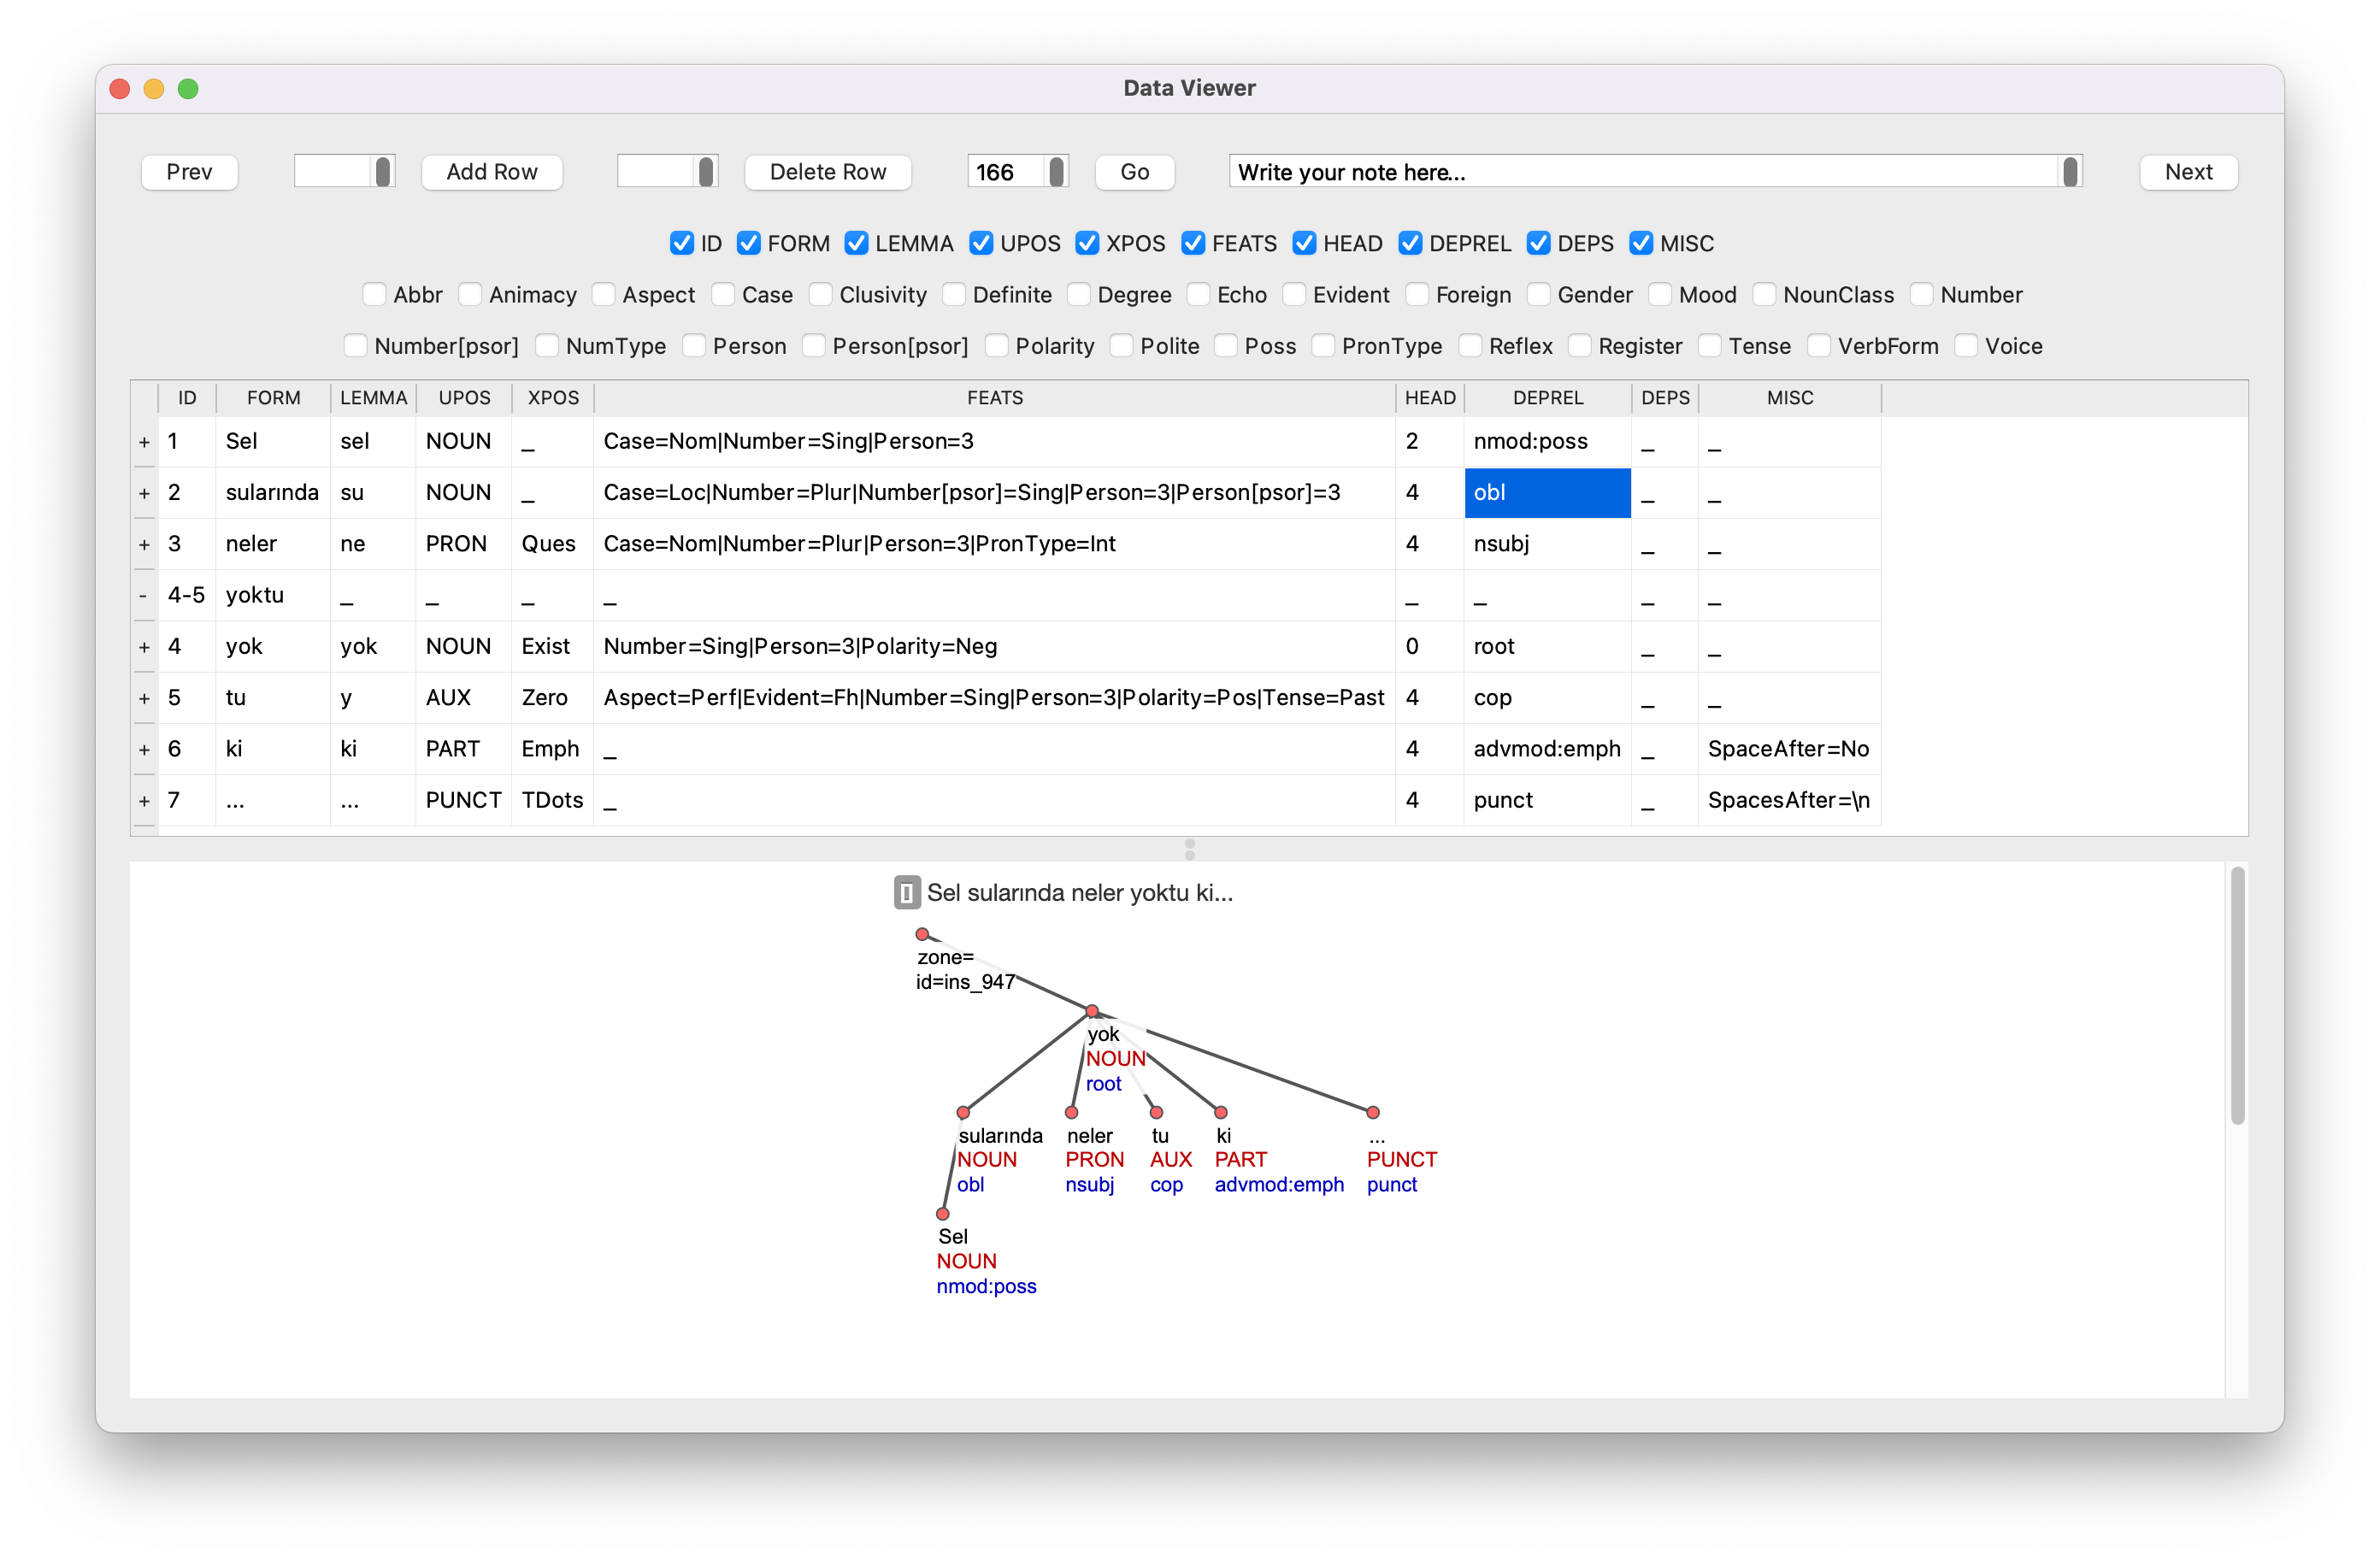
\includegraphics[width=0.8\textwidth]{figures/boat-v1-march-sample-annotation-mac.png}
        \caption{The annotation screen on \boatvone, captured while the sentence ``Sel sularında neler yoktu ki...'' is being annotated.}
        \label{fig:anno-fig-v1}
\end{figure}

\boatvone\ supports viewing features and their values individually under their corresponding columns (e.g. Case=Nom\textbar Number=Sing\textbar Person=3 can be shown in columns ``Case'', ``Number'', and ``Person'' with the values ``Nom'', ``Sing'', and ``3'').
It also allows the annotators to be able to take notes for specific annotations.

\subsection{Challenges of Agglutinative Languages}
\label{sec:challenges}
Agglutinative languages allow stacking multiple morphemes on a single root or stem to convey a wide range of linguistic information such as tense, aspect, number, person, possessor, and more.
Analytic languages, on the other hand, convey the same information through often free-standing function words.
A clear illustration of this contrast can be observed in \hyperref[trex]{Sentence (1)}: Each lemma of the Turkish sentence stacks at least two inflectional or derivational morphemes that carry out the function of free-standing morphemes in the corresponding English sentence.
Hence, the Turkish sentence has only 3 forms \textit{(masadaki, kitaplarını, görmüştüm)} while its English translation has 10 forms \textit{(I, had, seen, your, books, that, were, on, the, table)}.

\ex.
\label{trex}
Masa-da-ki \hspace*{.573cm}kitap-lar-ın-ı \hspace*{1.8cm}gör-müş-tü-m.\\
table-{\sc \Loc-\Der} book-{\sc \Pl-\Poss.\Second\Sg-\Acc} see-{\sc \Ant-\Pst-\First\Sg}\footnote{\printglossaries}\\
\textit{`I had seen your books that were on the table.'}

As a result of this contrast, lemmas in agglutinative languages like Turkish bear more features in the \feats\ column compared to analytic languages like English.
In addition to a higher feature-per-token count, agglutinative languages often have higher non-unique feature counts as well due to their rich repository of derivational and inflectional morphemes.

In order to offer an empirical example of this contrast, we compared non-unique features, total tokens, and features-per-token counts of multilingual \ud\ treebanks (ATIS and PUD)~\cite{atis-tr, atis-en, pud-tr, pud-en}.
Despite following different annotation customs, both Turkish treebanks have significantly higher non-unique features and lower token counts than their English counterparts (see \hyperref[table:feat-comp]{Table 1}).
As a result, both Turkish treebanks have more features per token; in fact, ATIS Turkish treebank has more than two times more features per token than ATIS English.

\newcolumntype{s}{>{\columncolor[HTML]{FFFAF0}} p{2.8cm}}
\begin{table}[h]
    \label{table:feat-comp}
    \centering
    \begin{tabular}{|s|>{\centering\arraybackslash} p{3.5cm}|>{\centering\arraybackslash} p{3cm}|>{\centering\arraybackslash} p{3cm}|}
       \hline
        \rowcolor[HTML]{FFFAF0} \multicolumn{4}{|c|}{\textbf{Comparison of \ud\ Treebanks}} \\ \hline\hline
        \multicolumn{1}{|c|}{\cellcolor[HTML]{FFFAF0} \textbf{Treebank}} & \textbf{Non-unique feats} & \textbf{Total tokens} & \textbf{Feats per token} \\\hline
        ATIS Turkish & 112,214 & 45,875 & 2.45 \\\hline
        ATIS English & 63,434 & 61,879 & 1.03 \\\hline
        PUD Turkish & 32,583 & 16,536 & 1.97 \\\hline
        PUD English & 23,995 & 21,176 & 1.13 \\\hline
    \end{tabular}
    \caption{Comparison of morphological feature annotations of Turkish and English \ud\ treebanks with equivalent sets of sentences in terms of meaning.}
\end{table}

In addition to having a higher feature count, being a free word order language makes annotating Turkish treebanks substantially challenging.
As Turkish allows scrambling and topicalization, the average dependency length per token in Turkish sentences is much higher than in fixed word order languages like English.
Moreover, such word order changing operations also affect headedness and the dependency arc direction while changing dependency lengths: The order of a dependent and its head can vary within or across the sentences (compare \hyperref[dep1]{Sentence 1} and \hyperref[dep2]{Sentence 2}).

\begin{multicols}{2}
\vspace*{\fill} 
\ex. \label{dep1}
\begin{dependency}
   \begin{deptext}
      Siyah \& kediyi \& ben \& gördüm \& sokakta \& . \\
   \end{deptext}
   \depedge{4}{3}{nsubj}
   \depedge{2}{1}{amod}
   \depedge{4}{2}{dobj}
   \depedge{4}{5}{obl}
   \depedge{4}{6}{punct}
\end{dependency} \\
Lit. The black cat I saw on the street. \\
\textit{‘I saw the black cat on the street.’} \\
\vspace{.05cm} \\
\textbf{Average arc length:} 1.4\\
\textbf{Longest arc length:} 3\\
\columnbreak

\ex. \label{dep2}
\begin{dependency}
   \begin{deptext}
      Gördüm \& sokakta \& siyah \& kediyi \& ben \& . \\
   \end{deptext}
   \depedge{1}{5}{nsubj}
   \depedge{1}{2}{obl}
   \depedge{4}{3}{amod}
   \depedge{1}{4}{dobj}
   \depedge{1}{6}{punct}
\end{dependency} \\
Lit. Saw on the street the black cat I. \\
\textit{‘I saw the black cat on the street.’} \\
\vspace{.05cm} \\
\textbf{Average arc length:} 2.8\\
\textbf{Longest arc length:} 5
%%% YOU NEED A NEW LINE BEFORE multicols -- SUZAN

\end{multicols}

An annotation interface designed for agglutinative languages must facilitate the annotator's job despite the changes in dependency length and arc direction.
As the dependency length increases, drag-drop interfaces become impractical since they require the annotator to drag lemmas for longer distances, thus decreasing the annotation speed and increasing the effort.
Moreover, the need to annotate more features per token also makes drag-drop interfaces very difficult to use for annotating agglutinative languages.
Thus, opting for an interface that utilizes the keyboard and allows typing is more practical for such languages.

In addition to the data entry method (the mouse vs the keyboard), feature-per-token counts, and changes in the dependency length and arc direction also require some adjustments in the interface.
For instance, the annotation interface must display the entire sentence and all lemma ids at all times.
This way, the annotator can see the head and/or dependent of the lemma that is being annotated even though they are dealing with a very verbose sentence or a very high dependency length.
Moreover, the annotation interface must be able to display large numbers of tags in the features column in an easy-to-read way so that the annotator can keep track of the annotation even when they are dealing with particularly packed lemmas.

% UD_English-ATIS/stats.xml:
% Non-unique feats: 63434
% Total tokens: 61879
% Feats per token: 1.0251296885857883

% UD_Turkish-ATIS/stats.xml:
% Non-unique feats: 112214
% Total tokens: 45875
% Feats per token: 2.4460817438692097

% UD_German-PUD/stats.xml:
% Non-unique feats: 56987
% Total tokens: 21000
% Feats per token: 2.7136666666666667

% UD_Turkish-PUD/stats.xml:
% Non-unique feats: 32583
% Total tokens: 16536
% Feats per token: 1.9704281567489115

% UD_Korean-PUD/stats.xml:
% Non-unique feats: 13430
% Total tokens: 16584
% Feats per token: 0.8098166907863

% UD_Spanish-PUD/stats.xml:
% Non-unique feats: 48819
% Total tokens: 22822
% Feats per token: 2.1391201472263606

% UD_Italian-PUD/stats.xml:
% Non-unique feats: 40715
% Total tokens: 22182
% Feats per token: 1.8354972500225408

% UD_French-PUD/stats.xml:
% Non-unique feats: 47560
% Total tokens: 24131
% Feats per token: 1.970908789523849

% UD_English-PUD/stats.xml:
% Non-unique feats: 23995
% Total tokens: 21176
% Feats per token: 1.1331224027200604

% explain comparison in table here

\section{Background}
\label{sec:background}

\subsection{BoAT-v1}
\label{sec:boatvone}

\boatvone~\cite{anon} is a standalone tool for annotating treebanks compatible with the \ud\ framework~\cite{ud}.
Although it was specifically developed for annotating Turkish treebanks, it supports agglutinative languages with rich morphologies; thus, it can be used for other languages as well.
It allows annotating one treebank at a time.
Annotations are stored in a file in the \conllu\ format.
The file is updated during the annotation process.
It uses a validation script developed by \ud\ to dynamically display errors to the annotator as they annotate.
\boatvone\ was used to create a manually annotated Turkish dependency treebank comprising 9,761 sentences from 5 different domains: essays, national newspapers, instructional texts, popular culture articles, and biographical texts.
It was implemented using Python~\cite{python} and Qt~\cite{qt}.

For annotation of any sentence, the annotator is shown a table which has a token per row with its corresponding columns (\id, \form, \udlemma, \upos, \xpos, \feats, \head, \deprel, \deps, and \misc\ as detailed in~\cite{anon}).
The annotator manually enters values for each column of each token.
It supports splitting and joining of lemmas.
This is particularly significant for agglutinative languages since their tokens are often comprised of multiple morphemes whose accurate annotations sometimes require adjusting lemma boundaries by splitting or merging.
Tokens that are split result in additional two rows whose lemmas are then manually adjusted by an annotator such that they become distinct parts of a token.
Figure~\ref{fig:anno-fig-v1} shows an annotation of a sentence.
The token ``yoktu'' (ID: 4-5) is split into ``yok'' (ID: 4) and ``tu'' (ID: 5).
Furthermore, with this split, the annotator divides the \feats\ column's value into individual morphological features for the lemmas with IDs 4 and 5.

\begin{figure}[th!]
    \centering
        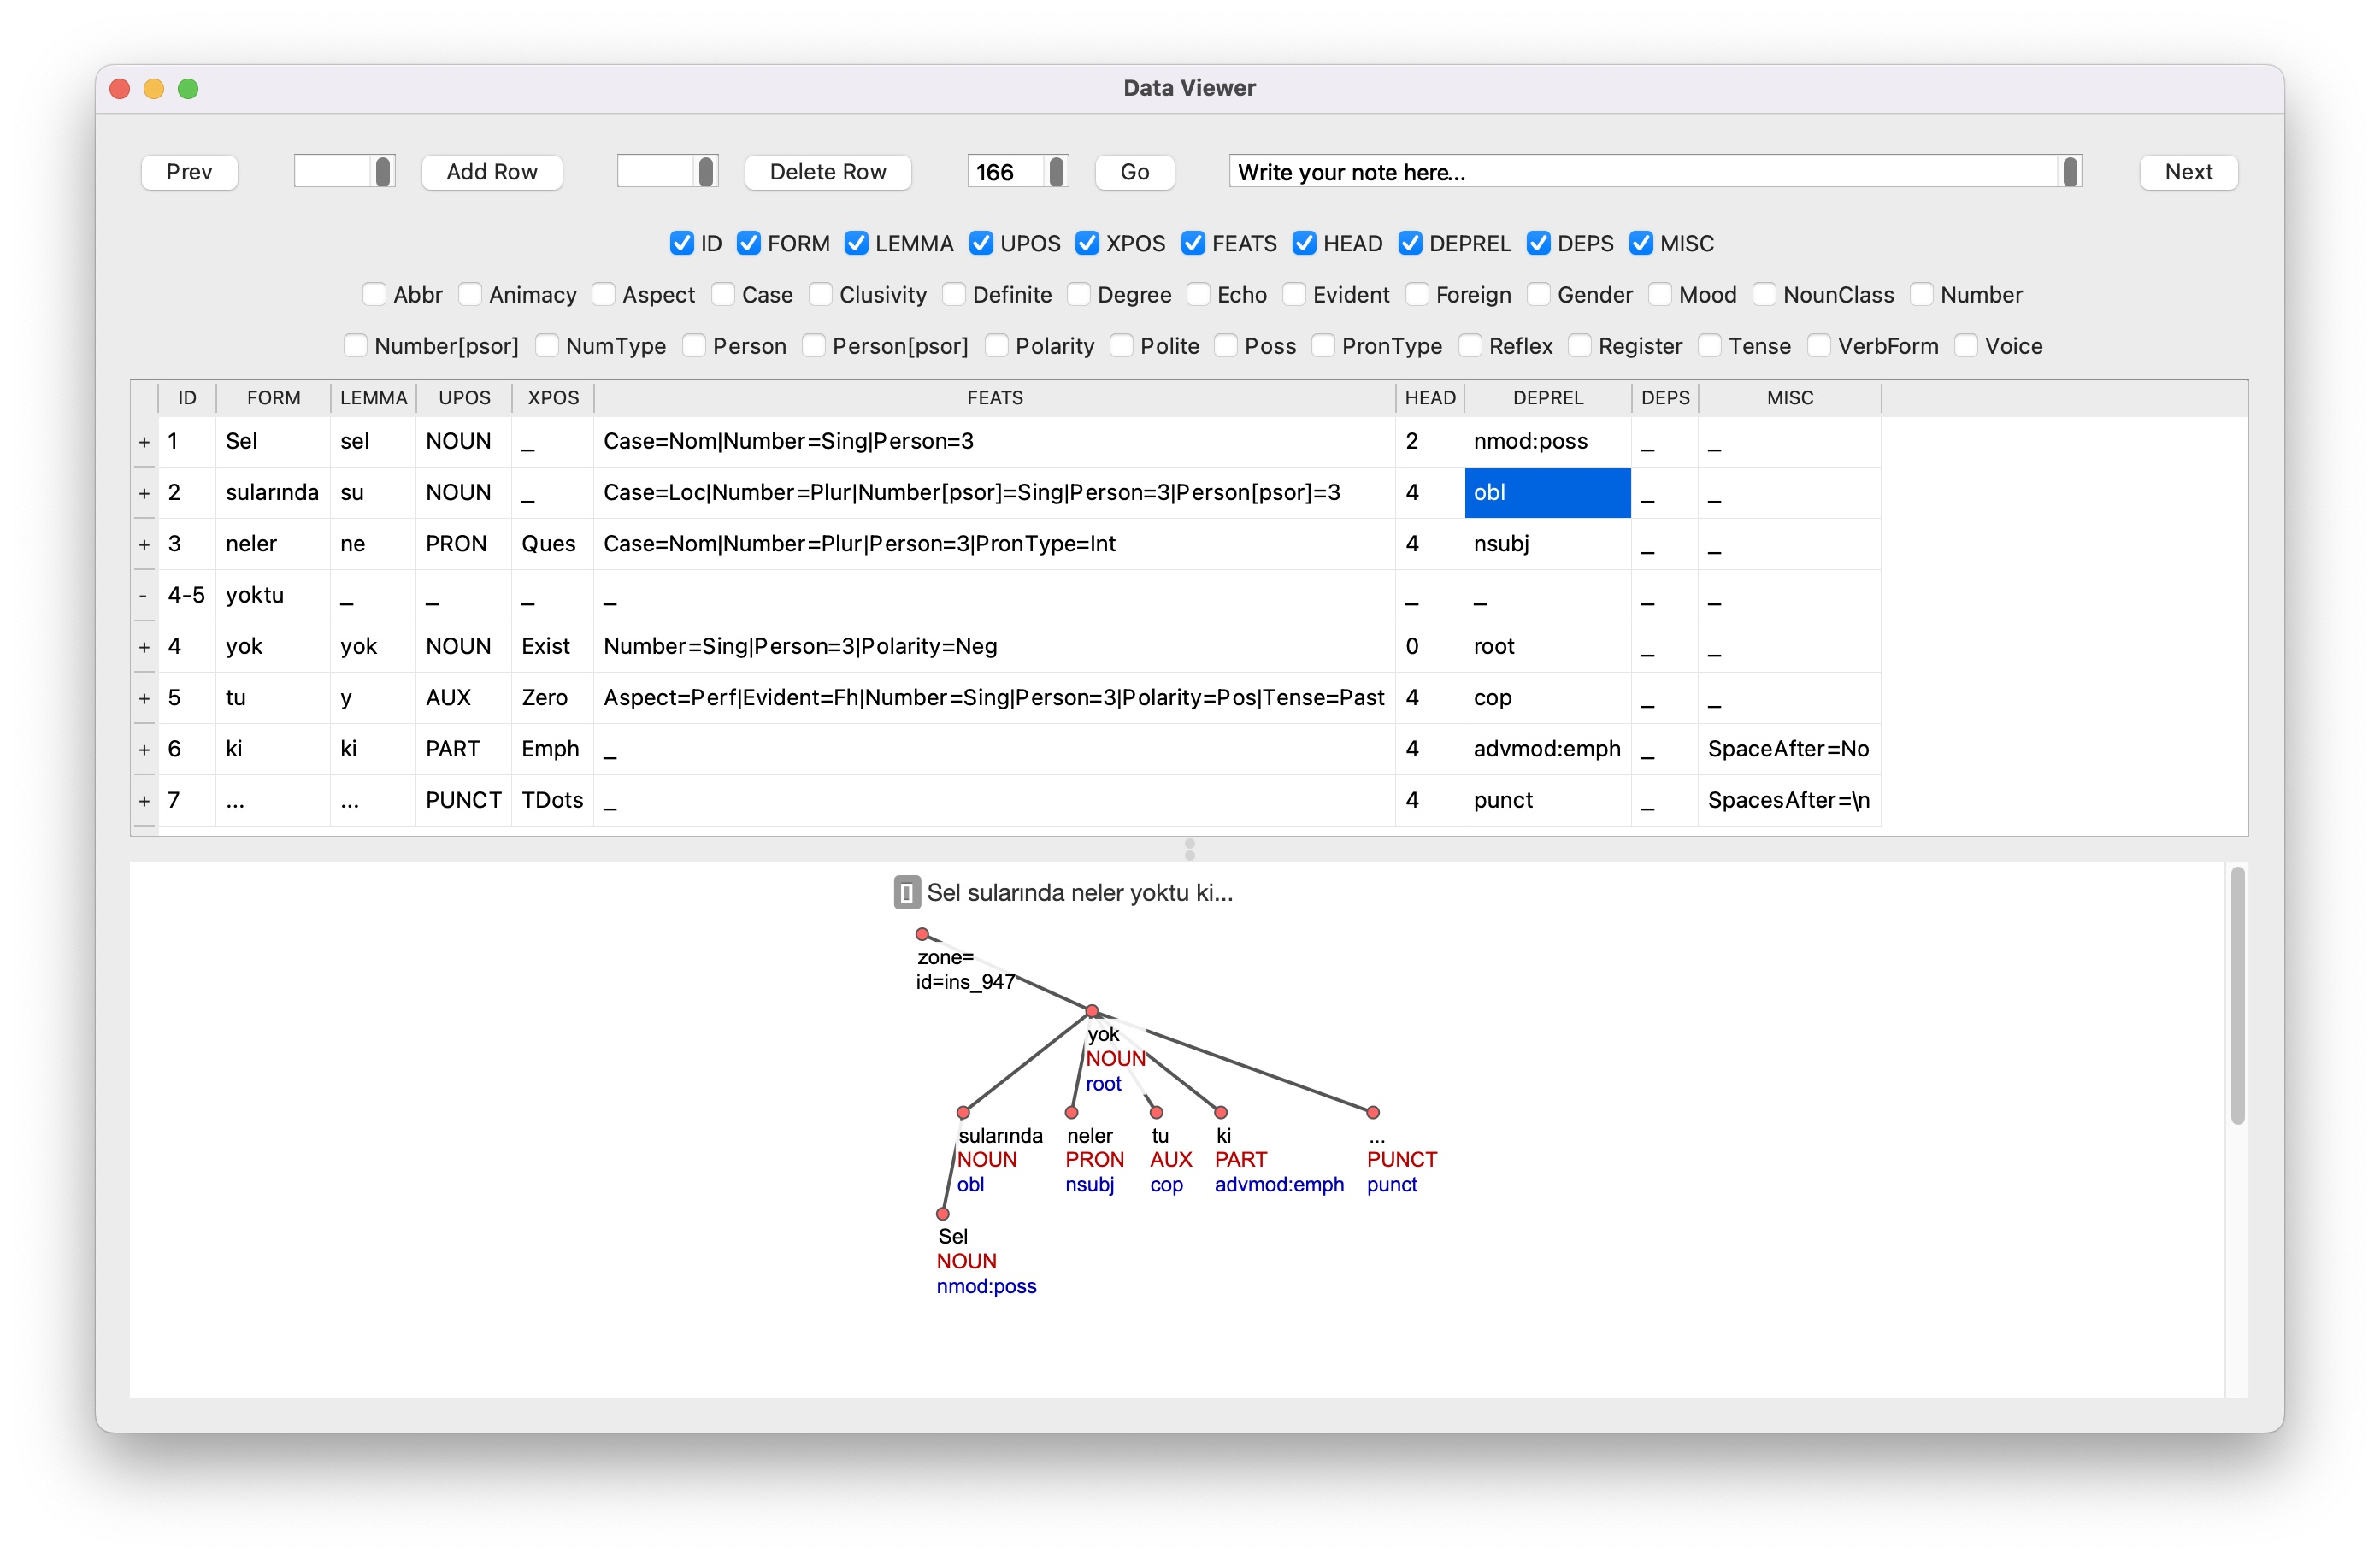
\includegraphics[width=0.8\textwidth]{boat-v1-march-sample-annotation-mac.jpg}
        \caption{The annotation screen on \boatvone, captured while the sentence ``Sel sularında neler yoktu ki...'' is being annotated.}
        \label{fig:anno-fig-v1}
\end{figure}

\boatvone\ supports viewing features and their values individually under their corresponding columns (e.g. Case=Nom\textbar Number=Sing\textbar Person=3 can be shown in columns ``Case'', ``Number'', and ``Person'' with the values ``Nom'', ``Sing'', and ``3'').
It also allows the annotators to be able to take notes for specific annotations.

\subsection{Challenges of Agglutinative Languages}
\label{sec:challenges}
Agglutinative languages allow stacking multiple morphemes on a single root or stem to convey a wide range of linguistic information such as tense, aspect, number, person, possessor, and more.
Analytic languages, on the other hand, convey the same information through often free-standing function words.
A clear illustration of this contrast can be observed in \hyperref[trex]{Sentence (1)}: Each lemma of the Turkish sentence stacks at least two inflectional or derivational morphemes that carry out the function of free-standing morphemes in the corresponding English sentence.
Hence, the Turkish sentence has only 3 forms \textit{(masadaki, kitaplarını, görmüştüm)} while its English translation has 10 forms \textit{(I, had, seen, your, books, that, were, on, the, table)}.

\ex.
\label{trex}
Masa-da-ki \hspace*{.6cm}kitap-lar-ın-ı \hspace*{1.65cm}gör-müş-tü-m.\\
table-{\sc \Loc-\Der} book-{\sc \Pl-\Poss.\Second\Sg-\Acc} see-{\sc \Ant-\Pst-\First\Sg}\footnote{\printglossaries}\\
\textit{`I had seen your books that were on the table.'}

As a result of this contrast, lemmas in agglutinative languages like Turkish bear more features in the \feats\ column compared to analytic languages like English.
In addition to a higher feature-per-token count, agglutinative languages often have higher non-unique feature counts as well due to their rich repository of derivational and inflectional morphemes.

In order to offer an empirical example of this contrast, we compared non-unique features, total tokens, and features-per-token counts of multilingual \ud\ treebanks (ATIS and PUD)~\cite{atis-tr, atis-en, pud-tr, pud-en}.
Despite following different annotation customs, both Turkish treebanks have significantly higher non-unique features and lower token counts than their English counterparts (see \hyperref[table:feat-comp]{Table 1}).
As a result, both Turkish treebanks have more features per token; in fact, ATIS Turkish treebank has more than two times more features per token than ATIS English.

\newcolumntype{s}{>{\columncolor[HTML]{FFFAF0}} p{2.8cm}}
\begin{table}[h]
    \label{table:feat-comp}
    \centering
    \begin{tabular}{|s|>{\centering\arraybackslash} p{3.5cm}|>{\centering\arraybackslash} p{3cm}|>{\centering\arraybackslash} p{3cm}|}
       \hline
        \rowcolor[HTML]{FFFAF0} \multicolumn{4}{|c|}{\textbf{Comparison of \ud\ Treebanks}} \\ \hline\hline
        \multicolumn{1}{|c|}{\cellcolor[HTML]{FFFAF0} \textbf{Treebank}} & \textbf{Non-unique feats} & \textbf{Total tokens} & \textbf{Feats per token} \\\hline
        ATIS Turkish & 112,214 & 45,875 & 2.45 \\\hline
        ATIS English & 63,434 & 61,879 & 1.03 \\\hline
        PUD Turkish & 32,583 & 16,536 & 1.97 \\\hline
        PUD English & 23,995 & 21,176 & 1.13 \\\hline
    \end{tabular}
    \caption{Comparison of morphological feature annotations of Turkish and English \ud\ treebanks with equivalent sets of sentences in terms of meaning.}
\end{table}

In addition to having a higher feature count, being a free word order language makes annotating Turkish treebanks substantially challenging.
As Turkish allows scrambling and topicalization, the average dependency length per token in Turkish sentences is much higher than in fixed word order languages like English.
Moreover, such word order changing operations also affect headedness and the dependency arc direction while changing dependency lengths: The order of a dependent and its head can vary within or across the sentences (compare \hyperref[dep1]{Sentence 1} and \hyperref[dep2]{Sentence 2}).

\begin{multicols}{2}
\vspace*{\fill} 
\ex. \label{dep1}
\begin{dependency}
   \begin{deptext}
      Siyah \& kediyi \& ben \& gördüm \& sokakta \& . \\
   \end{deptext}
   \depedge{4}{3}{nsubj}
   \depedge{2}{1}{amod}
   \depedge{4}{2}{dobj}
   \depedge{4}{5}{obl}
   \depedge{4}{6}{punct}
\end{dependency} \\
Lit. The black cat I saw on the street. \\
\textit{‘I saw the black cat on the street.’} \\
\vspace{.05cm} \\
\textbf{Average arc length:} 1.4\\
\textbf{Longest arc length:} 3\\
\columnbreak

\ex. \label{dep2}
\begin{dependency}
   \begin{deptext}
      Gördüm \& sokakta \& siyah \& kediyi \& ben \& . \\
   \end{deptext}
   \depedge{1}{5}{nsubj}
   \depedge{1}{2}{obl}
   \depedge{4}{3}{amod}
   \depedge{1}{4}{dobj}
   \depedge{1}{6}{punct}
\end{dependency} \\
Lit. Saw on the street the black cat I. \\
\textit{‘I saw the black cat on the street.’} \\
\vspace{.05cm} \\
\textbf{Average arc length:} 2.8\\
\textbf{Longest arc length:} 5

\end{multicols}

An annotation interface designed for agglutinative languages must facilitate the annotator's job despite the changes in dependency length and arc direction.
As the dependency length increases, drag-drop interfaces become impractical since they require the annotator to drag lemmas for longer distances, thus decreasing the annotation speed and increasing the effort.
Moreover, the need to annotate more features per token also makes drag-drop interfaces very difficult to use for annotating agglutinative languages.
Thus, opting for an interface that utilizes the keyboard and allows typing is more practical for such languages.

In addition to the data entry method (mouse versus keyboard), feature-per-token counts, and changes in the dependency length and arc direction also require some adjustments in the interface.
For instance, the annotation interface must display the entire sentence and all lemma ids at all times.
This way, the annotator can see the head and/or dependent of the lemma that is being annotated even though they are dealing with a very verbose sentence or a very high dependency length.
Moreover, the annotation interface must be able to display large numbers of tags in the features column in an easy-to-read way so that the annotator can keep track of the annotation even when they are dealing with particularly packed lemmas.

% \section{Related Work}
\label{sec:related}

Annotation tools may be characterized in terms of their accessibility and the support they provide for languages, various annotation categories, user interface modalities, standards, and multiple annotators.
Adherence to standards is recommended to get the most benefit from the annotated data sources.
Universal Dependencies~\cite{UD} is an actively growing standard that intends to cover all languages and its support for agglutinative languages is evolving.

Several dependency annotation tools have been proposed such as \textit{brat}~\cite{brat}, \textit{UD Annotatrix}~\cite{tyers-etal:2018} and \textit{DgAnnotator}~\cite{dgannotator,UD-tools}.
These tools are not developed for a specific language, but can be used with a variety of languages.
They mostly rely on mouse-based user interaction, which is inefficient for annotating agglutinative languages due to the need for extensive annotation for most tokens.

The ITU Treebank Annotation Tool~\cite{pamay-etal-2015-annotation} was developed for Turkish and has been used to annotate the ITU Web Treebank~\cite{itu-web-tb}.
It was written in Java as an open-source standalone tool and has several versions.
It has 3 three stages of annotation: morphological analysis, morphological disambiguation and syntax analysis.
It offers semi-automated support for annotators through analyzers for creating new datasets as well as correcting already existing Turkish treebanks.
It mostly relies on mouse-based interactions and doesn't support the \ud\ framework.

WebAnno~\cite{webanno} is a web-based open-source annotation tool, that is not restricted to dependency annotations but has support for morphological, syntactical, and semantic annotations also, with multi-user support.
To annotate features of a token, it requires several mouse clicks which is impractical for MRLs.
It does not display a dependency graph, unlike \boatvone\ and \boatvtwo.
It presents several sentences simultaneously, which can be distracting.

\boatvtwo\ is the second iteration of \boatvone.
It improves on it by including a search functionality, a database to represent sentences in a more essential way rather than a plaintext file and an accessible web interface with an API for flexibility.
\boatvtwo\ has been developed to reduce clutter that \boatvone\ was found to have in some spaces by the feedback of \boatvone.

\section{Related Work}
\label{sec:related}

Annotation tools can be categorized in terms of their accessibility, and the support they provide for different languages, various annotation frameworks, user interface modalities, annotation-related standards, multiple annotators, searching of annotations, and automation.
Adherence to standards is recommended to get the most benefit from the annotated language resources.
Universal Dependencies~\cite{ud} (\ud) is an actively growing standard for the annotation of treebanks, intending to cover all languages, and its support for agglutinative languages is evolving.

Numerous dependency annotation tools have been developed with many of them being \ud-compliant, such as brat~\cite{brat}, UD Annotatrix~\cite{ud-annotatrix}, and DGA~\cite{dgannotator}.
Most of these tools are capable of annotating a variety of languages and all the tools that are detailed below do so.
Most tools require mouse-based user interactions, which is inefficient for the annotation of agglutinative languages due to several reasons, including the need for extensive annotation for most tokens.

% 2011
ITU Treebank Annotation Tool~\cite{itu-annotation-tool} is an open-source standalone tool, developed specifically for Turkish.
It has three stages of annotation: morphological analysis, morphological disambiguation, and syntax analysis.
It offers semi-automated support for annotators through analyzers for creating new datasets as well as correcting already existing Turkish treebanks.
It mostly relies on mouse-based interactions and doesn't have support for the \ud\ framework.
This tool has been used to annotate the ITU Web Treebank~\cite{itu-annotation-tool}. % same ref with tool
It has three versions, and its latest version (3) was written in Java, requiring Java to be installed on the system used for annotations.

% 2012
brat~\cite{brat} is a web-based \textit{text} annotation tool which provides a collaborative annotation environment.
Being web-based, it's usable across different platforms.
It's very flexible in its annotation types and has support for many annotation tasks such as dependency, entity, or coreference annotation.
This tool is also used for the visualization of annotations.
Annotators use a mouse and keyboard together to annotate.
Annotators are able to transfer their annotations in a file format called \textit{standoff} specific to brat.
It is configurable to support annotations compliant with \ud\ and is used for visualization in \ud's own documentation system.
brat supports real-time collaboration, even allowing annotators to edit the same annotation.
It supports searching the documents or their annotations through using various filters.

% 2015
The Dependency Grammar Annotator~\cite{dgannotator} (also known as DGA or DgAnnotator) is a dependency annotation tool.
It enables its users to annotate POS and dependency relation tags via mouse clicks.
It supports the transfer of annotations in \ud-compliant formats.
It doesn't support multiple annotators to work on the same treebank.
There is no search functionality.
It was written in Java~\cite{java} and consequently requires Java.

% 2016
WebAnno~\cite{webanno} is a web-based open-source annotation tool, that is not restricted to dependency annotations but has support for morphological, syntactical, and semantic annotations also, with multi-user support.
To annotate the morphological features of a token, it requires several mouse clicks which is impractical for MRLs.
The sentences to be annotated are displayed vertically on a single screen, unlike many tools that focus on a single sentence at a time.
It supports the curation of annotations created by multiple annotators.
It has two installment options, standalone and server.
The standalone version requires Java, while the server version requires a Tomcat~\cite{tomcat} server with a MySQL~\cite{mysql} database.

% 2018
UD-Annotatrix~\cite{ud-annotatrix} is a \ud-specific dependency annotation tool that aims to be simpler than brat.
Mouse usage is necessary, in addition to keyboard entries, for annotation.
It supports real-time collaboration if the tool is deployed in a server.
It employs annotation standards of \ud\ and CG3~\cite{cg3}.
It doesn't have a search functionality.

% 2019
CoNLL-U Editor~\cite{conll-u_editor} is a web-based annotation tool, specific to the \conllu~\cite{conll} format of \ud.
It saves every edit of annotations by version control.
If specific lists of part-of-speech tags are provided by the annotators, it supports auto-completion during annotation.
Multiple annotators are able to annotate the same treebank if they don't work on the same sentence at a time.
Annotators can search using any combination of linguistic tags of \ud\ using the tool.
It requires a Java-based server.

% 2022
StarDust~\cite{stardust} is a recent standalone dependency annotation tool.
It uses 2 layers: morphological disambiguation and dependency annotation layers, sequentially.
In the dependency annotation layer, annotators are expected to click on a dependent and drag the cursor to its head.
It stores each sentence's annotation in a different file.
For backups of the annotations, it uses Dropbox~\cite{dropbox}, which is a proprietary cloud storage platform.
There were several treebanks annotated using this tool: 1 English and 5 Turkish treebanks.

BoAT-v2 is the second iteration of \boatvone.
It improves on it by including a search functionality, an auto-completion feature, a database to represent sentences in a more essential way rather than a plaintext file, multiple dependency graph visualization options, and a web interface with an API for flexibility and accessibility.
\boatvtwo\ also reduces the clutter that \boatvone\ was reported to have in parts of the screen in the feedback of the previous \boatvone\ usage.

\begin{table}[ht]
    \label{table:rel-work}
    \centering
    \begin{tabular}{|s|>{\centering\arraybackslash} p{1.1cm}|>{\centering\arraybackslash} p{1.6cm}|>{\centering\arraybackslash} p{2.4cm}|>{\centering\arraybackslash} p{1.9cm}|>{\centering\arraybackslash} p{1.2cm}|}
       \hline
        \rowcolor[HTML]{FFFAF0} \multicolumn{6}{|c|}{\textbf{Comparison of Annotation Tools}} \\ \hline\hline
        \multicolumn{1}{|c|}{\cellcolor[HTML]{FFFAF0} \textbf{Tool}} & \textbf{Mouse} & \textbf{Keyboard} & \textbf{Standards} & \textbf{Multi-user} & \textbf{Search} \\\hline
        brat & + & + & Extendable & + & + \\\hline
        UD Annotatrix & + & + & \ud\ \& CG3 & + & - \\\hline
        DgAnnotator & + & - & \ud\ & - & - \\\hline
        CoNLL-U Editor & + & + & \ud\ & + & + \\\hline
        ITU & + & + & \ud\ & - & - \\\hline
        WebAnno & + & + & \ud\ & + & - \\\hline
        StarDust & + & + & - & - & - \\\hline
        \boatvtwo\ & + & + & \ud\ & + & + \\\hline
    \end{tabular}
    \caption{Properties of the above-mentioned annotation tools, namely whether they support mouse or keyboard usage, what standards they abide by, and whether they support multi-annotator treebanks or a search functionality.}
\end{table}

% \section{Requirements and Design}
\label{sec:requirements}

% Suzan, introduction sentence
In-depth interviews and requirements elicitation with annotators that have annotated the entire \bountreebank{}, which has close to 10 thousand sentences, have been conducted to elicit the software requirements.
Annotators may struggle with a specific annotation and want to be able to search for specific annotations similar to the one they are currently doing to make the treebank consistent within itself and reduce their cognitive load in general.
Thus, a search functionality for annotators needs to be built with a network of annotators to allow them to cross-check each other's work.
Because there was a pressing need for a network, we decided to develop a new web-based tool from scratch.

The annotation process requires a great deal of attention, therefore, the main priority is to improve the user experience for the annotator so that they can more efficiently produce accurate annotations.
Annotators use the tools sometimes for hours on end.
Software should make the work easier by reducing distractions and automating work that can be automated.
One of the requirements we have gathered for not breaking the focus of the annotator is for the software to use only keyboard for every task.
\boat{} is a keyboard-oriented application.
User should not have to use a mouse for any type of task.
Since users lose focus after some time naturally, automating the entries and checking errors are high priorities in this respect.
Autocomplete should be provided for parts of the annotation where it is known what values are allowed for a \conllu{} type annotation.
Autocompletion reduces errors and increases efficiency.

One feature requested by annotators is using the screen space in a compact manner and removing any clutter that's not used much.
Considering this, the previous application's checkboxes have been converted into a dropdown menu, leaving more space for the annotation table where most of the annotator focus is directed towards.

A search API for the annotation database of the treebanks is another requirement.
An annotator should be able to search the treebank they are a part of to see other annotations done for a specific sentence or go to a sentence's annotation page to start annotating.
Sometimes a user may not be sure of an annotation and would like to consult previous annotations for similar cases.
They should be able to search the database in a complex way, by case, features or direct text, etc.
An outsider also should be able to use the API to get the annotations of a particular treebank to use in their tasks in a systematic way.

Following good software practices, this tool should be dockerized and made available as open source.

\section{Requirements and Design}
\label{sec:requirements}

Requirements elicitation and validation meetings were held with annotators who worked on a treebank~\cite{anon} involving thousands of sentences to identify the software requirements.
The main requirements that emerged are:
\begin{itemize}[before=\normalfont, font=\itshape, align=left,noitemsep,topsep=0pt,parsep=3pt,partopsep=0pt,labelsep=3pt,align=left]
    \item[Support for sentence annotation:]
        To ensure speedy and accurate annotations, various features must be provided.
        In order to eliminate mistakes caused by typos while saving time for the annotator, \textit{auto-completion} should be supported whenever possible.
        Due to typologies of and syncretism being generally higher in MRLs, automatic parsing of such treebanks is difficult and they more often than not fail to create valid parsings of tokens.
        Thus, refining automatic parsing becomes an important task for agglutinative languages.
        Words in MRLs tend to have morphemes stacked on roots.
        Annotators must be able to refine or correct automatically parsed entries, which for agglutinative languages includes splitting or joining of lemmas.
    \item[Use of screen real estate and customization:]
        Annotators annotate many sentences in each session.
        For agglutinative languages, sentences tend to be long and complicated.
        The view of such sentences can cover a considerable part of the screen.
        The annotator must focus on the sentence being annotated, the lemmas, and all the features, which require lots of concentration.
        The annotation process must require little to no scrolling.
        For particularly long sentences, no scrolling may not be possible; however, the sentence being annotated should always be in sight of the annotator.
        Furthermore, every annotator has their unique preferences regarding how they would like to annotate.
        They must have some control on showing or hiding certain information according to their preferences.
        Overall, efficient use of screen real estate is important to provide the context needed to annotate long sentences.
    \item[Keyboard-oriented input:]
        Annotations of agglutinative languages require annotation of several morphological features for many tokens of a sentence in comparison to analytic languages like English.
        While drag-drop interfaces can work well for analytic languages, they don't for MRLs as they require more toggles between mouse and keyboard interactions which becomes frustrating.
        Keyboard-based interaction must be offered for all possible tasks so that the annotator can work without needing to switch between the keyboard and the mouse.
    \item[Collaborative annotation:]
        The large sizes of treebanks necessitate that they be annotated by multiple annotators.
        The tool must support multiple annotators working simultaneously on the same treebank.
        The ability to share annotations is vital for reference and consistency.
        Hence, the tool must provide a means for registering multiple annotators and keeping track of their respective annotations.
    \item[Search:]
        During the annotation of a sentence, annotators sometimes need to refer to previous annotations for guidance.
        An annotator should be able to search a treebank according to surface forms, and importantly, according to linguistic features.
        They should be able to perform complex searches that involve several criteria such as \ud\ tags, individual morphological features, and surface forms.
        This requirement reduces cognitive load and facilitates consistency among annotations.
\end{itemize}

Given these requirements, we decided that a web-based application that supports multiple authenticated users would be able to provide a collaborative platform for annotators.
The treebank and user annotations persists in a database which makes managing the data and searches much more reliable and efficient.
Also, an API is developed to support flexibility and extensibility.
Finally, in addition to making the tool open-source, we containerized the application using Docker~\cite{docker} to support its accessibility.

% \section{Implementation}
\label{sec:implementation}

Web application development framework \textit{Django}~\cite{django}, Web API toolkit \textit{Django REST Framework} (DRF)~\cite{drf} and Python~\cite{python} library \textit{django-filter}~\cite{django-filter} are used to operate \boatvtwo.
PostgreSQL~\cite{psql} is used to provide a database for the server-side applications of the software.
During the implementation phase, decisions regarding models of the database have been directed towards the UI utilizing the API for database queries and searches.
The models reflect the \ud\ format of sentences and annotations are saved as fields of word lines.

All the pages of the tool have been supported by Bootstrap~\cite{bootstrap}.
The annotation page has most of the functionalities of \boatvone.
Entries are validated and errors are displayed on the annotation page for annotators to see invalid edits in real time, according to the \ud\ framework~\cite{UD} and the language provided.

Python library \textit{spa\textsc{C}y}~\cite{spacy} is used to provide linear dependency graphs.
Another JavaScript-based linear dependency graph~\cite{spyssalo} making use of \textit{brat}~\cite{brat} is used to provide graphs as well.
An annotator's preference regarding this may vary, thus, giving them visualization options is important.

\begin{figure}[tbh]
    \centering
    \frame{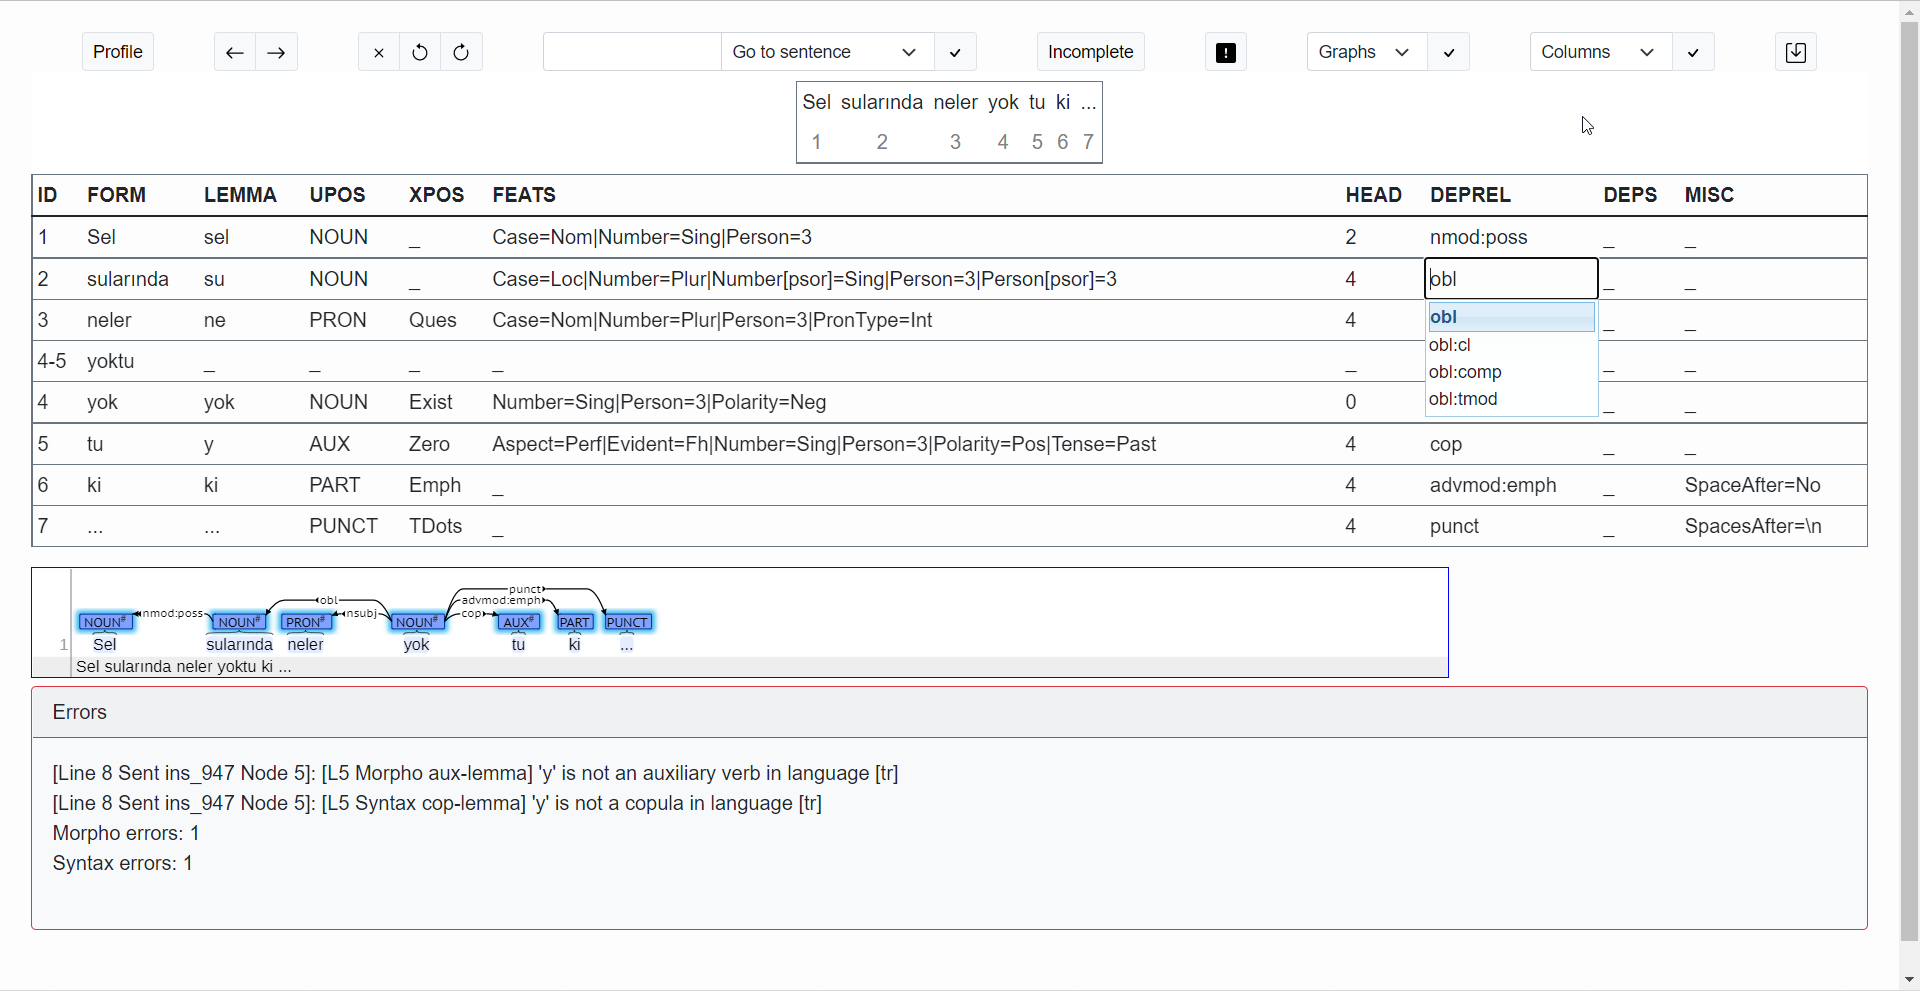
\includegraphics[width=1\textwidth]{figures/sample-annotation.png}}
    \caption{The annotation screen for the sentence ``Sel sularında neler yoktu ki...''.
        The annotator is choosing an annotation for the \deprel\ tag of the \form\ ``sularında''.
        The valid alternatives pop up based on the entry and can be selected via use of arrows. }
    \label{fig:anno-fig}
\end{figure}

\subsection{Features}
\label{sec:features}

There are many new features and improvements in this tool, as well as most of the functionality of \boatvone.

\begin{itemize}[before=\normalfont, font=\itshape, align=left]
    \item[Treebanks:]
        Multiple treebanks, with each one having its own sets of sentences, can be created in a single deployment.
        When uploading a file, a treebank is selected.

    \item[Loading files:]
        Instead of loading a dataset file before every annotation session, a \conllu\ file is uploaded to the database.
        The file is rejected if incorrectly formatted, otherwise uploaded to the database.
        This way, other annotators working with the same treebank don't have to provide the same file.

    \item[Annotation view:]
        The annotation page is very similar to the one on \boatvone~\cite{trk2020resources}, as seen in Figure~\ref{fig:anno-fig}.
        There is an annotation table for annotating fields in word lines of sentences.
        It also includes a dependency graph and an error card, both of which are in sync with the edits done on the table cells.
        Three different dependency graph representations are provided in this tool.
        Two of the graphs, which are both horizontal and linear, have been selected due to space considerations.
        The error card displays errors for the current annotation, validating it via the UD validation script.

    \item[Network-enabled search:]
        An important feature in this version is the ability to cross-check annotations by implementing a network for annotators where they can review the annotations done by other annotators.
        This can be helpful and a learning experience for annotators.

        For example, the annotator of the \bountreebank was annotating a sentence with a Zodiac sign noun.
        Not being sure of how to annotate its \upos\ tag, she searched the \conllu\ file manually for similar cases and encountered two different values with which nouns of Zodiac signs were annotated previously.
        Besides not helping how to choose a \upos\ tag, this raises a consistency issue within the treebank as well.
        This task could have been handled by a search of the database.
        We provide a search page and an API in this tool with which treebanks can be searched by \ud\ tags.

        Another example could be given by the various \textit{-ki} morphemes in Turkish.
        In the sentence ``Evdeki halılar yıkandı.'' (\textit{The rugs at home were washed.}), the \textit{-ki} acts as an adjectivizer.
        However, in ``Benim halılarım yün, Ayşeninkiler sentetik.'' (\textit{My rugs are woolen. Ayşe's are synthetic.}), it is pronominal.
        An annotator might not recall how a specific \textit{-ki} morpheme should be annotated, which can be remedied with a simple search.
        Annotators have informed us that such cases occur frequently when annotating MRLs.

        The inter-annotator agreement allows us to see some anomalies in the Turkish part of the \ud\ framework.
        For example, if a sentence were annotated a way by many annotators but the \ud\ validation script were finding it invalid, this might indicate the validation were lacking in this respect of the Turkish language.

    \item[Annotation status:]
        There are 3 annotation statuses ("Incomplete", "Draft" and "Complete") and they are cycled through by the annotator in the annotation view.
        Status of an annotation is also shown in the search view, helping to select an appropriate case.
        There is another view where completed, drafted or incomplete annotations can be listed.

\end{itemize}

\section{Implementation}
\label{sec:implementation}

The annotation tool is implemented using Python~\cite{python}, the web application development framework \textit{Django}~\cite{django} and the API framework \textit{Django REST Framework} (DRF)~\cite{drf}.
The webpages use Bootstrap~\cite{bootstrap}.
PostgreSQL~\cite{psql} is used as the database management system.
The database models are in line with the \ud\ format of sentences.
Annotations are validated according to the \ud\ guidelines and errors are reported on the annotation page.
Three alternative forms of dependency graph visualizations are supported, two of which are newly added, compact and horizontal to reduce the required screen real estate~\cite{spacy,spyssalo}.

The following features have been implemented in order to support the creation of valid annotations with increased speed in a collaborative manner:
\begin{itemize}[before=\normalfont, font=\itshape, align=left,noitemsep,topsep=0pt,parsep=3pt,partopsep=0pt,labelsep=3pt,align=left]
    \item[Treebank handling:]
        The tool should support the annotation of multiple treebanks.
        \boatvtwo\ uses a database to persist the annotations of multiple annotators of multiple treebanks.
        After annotations are done, annotators can export their annotations as an annotation file in the \conllu\ format of \ud.

    \item[Sentence annotation:]
    	A sentence is selected by a user in order to annotate.
        The annotation page consists of three main parts: (1) A table with rows for each token of a sentence and columns, which represent the \ud\ tags of a sentence, corresponding to their annotations; (2) the dependency graph of the sentence; and (3) validation results according to the \ud\ guidelines.
        The dependency graph and errors are updated with the annotations.
        Several dependency graph representations are supported to serve the annotator's preference.
        Two horizontal dependency graphs are supported since vertical graphs can consume a significant amount of screen real estate, which leads to loss of focus in long sentences commonly found in agglutinative languages.
        One vertical tree-like dependency graph is also supported in case the annotator would like to see the tree structure of the annotation.

        An annotator may need to stop the annotation of a sentence due to sentence complexity or external interruptions.
        To capture the state of an annotation, status is used with values of ``New", ``Draft" and ``Complete".
        The status of a sentence that has not yet been annotated is ``New''.
	    Annotators set their annotation statuses to ``Draft'' or ``Complete''.

        The annotator is able to perform most operations via keyboard action, based on the demand of the annotators (see Section~\ref{sec:requirements} for details).
        Upon the experience of annotating a Turkish treebank with \boatvone, the annotators were pleased with the convenience and speed keyboard-based interaction provided them with.

    \item[Searching for reference and consistency:]
        To facilitate effective searching, a search functionality has been implemented in \boatvtwo.
        Users are able to search for previously annotated sentences by any annotator based on combinations of surface text and \ud\ tags (e.g. morphological features) with regular expression support.
        This feature supports annotators to share their annotations, which consequently is expected to result in more valid and consistent treebanks.
		Without a search feature, an annotator would have to manually search their annotation files for relevant cases (e.g. how to annotate a certain surface form's \upos\ tag).
		The form might have been annotated in various ways throughout the treebank, alas it is highly unlikely that a manual search would reveal this inconsistency.
		In this case, the annotator would likely use the first usage they come across as their reference.
        This problem gets more complicated for syncretic morphemes such as \textit{-ki} in Turkish.
        For instance, in the sentence ``Evdeki halılar yıkandı.'' (\textit{The rugs at home were washed.}), the \textit{-ki} acts as an adjectivizer.
        However, in ``Benim halılarım yün, Ayşeninkiler sentetik.'' (\textit{My rugs are woolen. Ayşe's are synthetic.}), it becomes pronominal.
        Searching for sentences where the morpheme \textit{-ki} occurs with basic text search of an annotation file would be unfruitful as there would be too many occurrences, owing to its role in the Turkish language's grammar and also brevity as a word.

    \item[Inter-annotator agreement:]
        The annotator consistency of a treebank is an indicator of the quality of the resulting resource.
        Inter-annotator agreement is done by computing the consistency among annotators.
        Since this tool keeps track of annotator actions, such computations are straightforward.
        Some visualizations shall accompany these statistics.

\end{itemize}

% \section{Annotation Procedure}
\label{sec:annotation}
This section describes how an annotator annotates a Turkish sentence.

An annotator selects a sentence from a treebank, which has previously uploaded sentences coming from a \conllu{} formatted file.
They fill the cells of the annotation table's fields.
During the annotation, an annotator can make use of dependency graphs, error cards and the search functionality.
Dependency graphs are visual cues for how an annotation is going, using HEADs and DEPRELs.
They can choose 3 different graphs one at a time or select to hide.
Different graphs show the same information with a horizontal or vertical tree.
Errors are helpful reminders, coming from a validation script found on the UD repository.
They can use the search functionality to search for previous annotations by other annotators or themselves, using various fields (text, FEATS, etc.) for the query.
By checking similar annotations, an annotator can ensure consistency and don't lose focus by trying manual methods for the same information.
When an annotation is done, they select the annotation to be "Complete".

\section{Using BoAT-v2}
\label{sec:annotation}

\begin{figure}
    \centering
    \tcbox[left=0mm,right=0mm,top=0mm,bottom=0mm,boxsep=1pt,arc=0mm,boxrule=0.5pt,colframe=Gray]
    {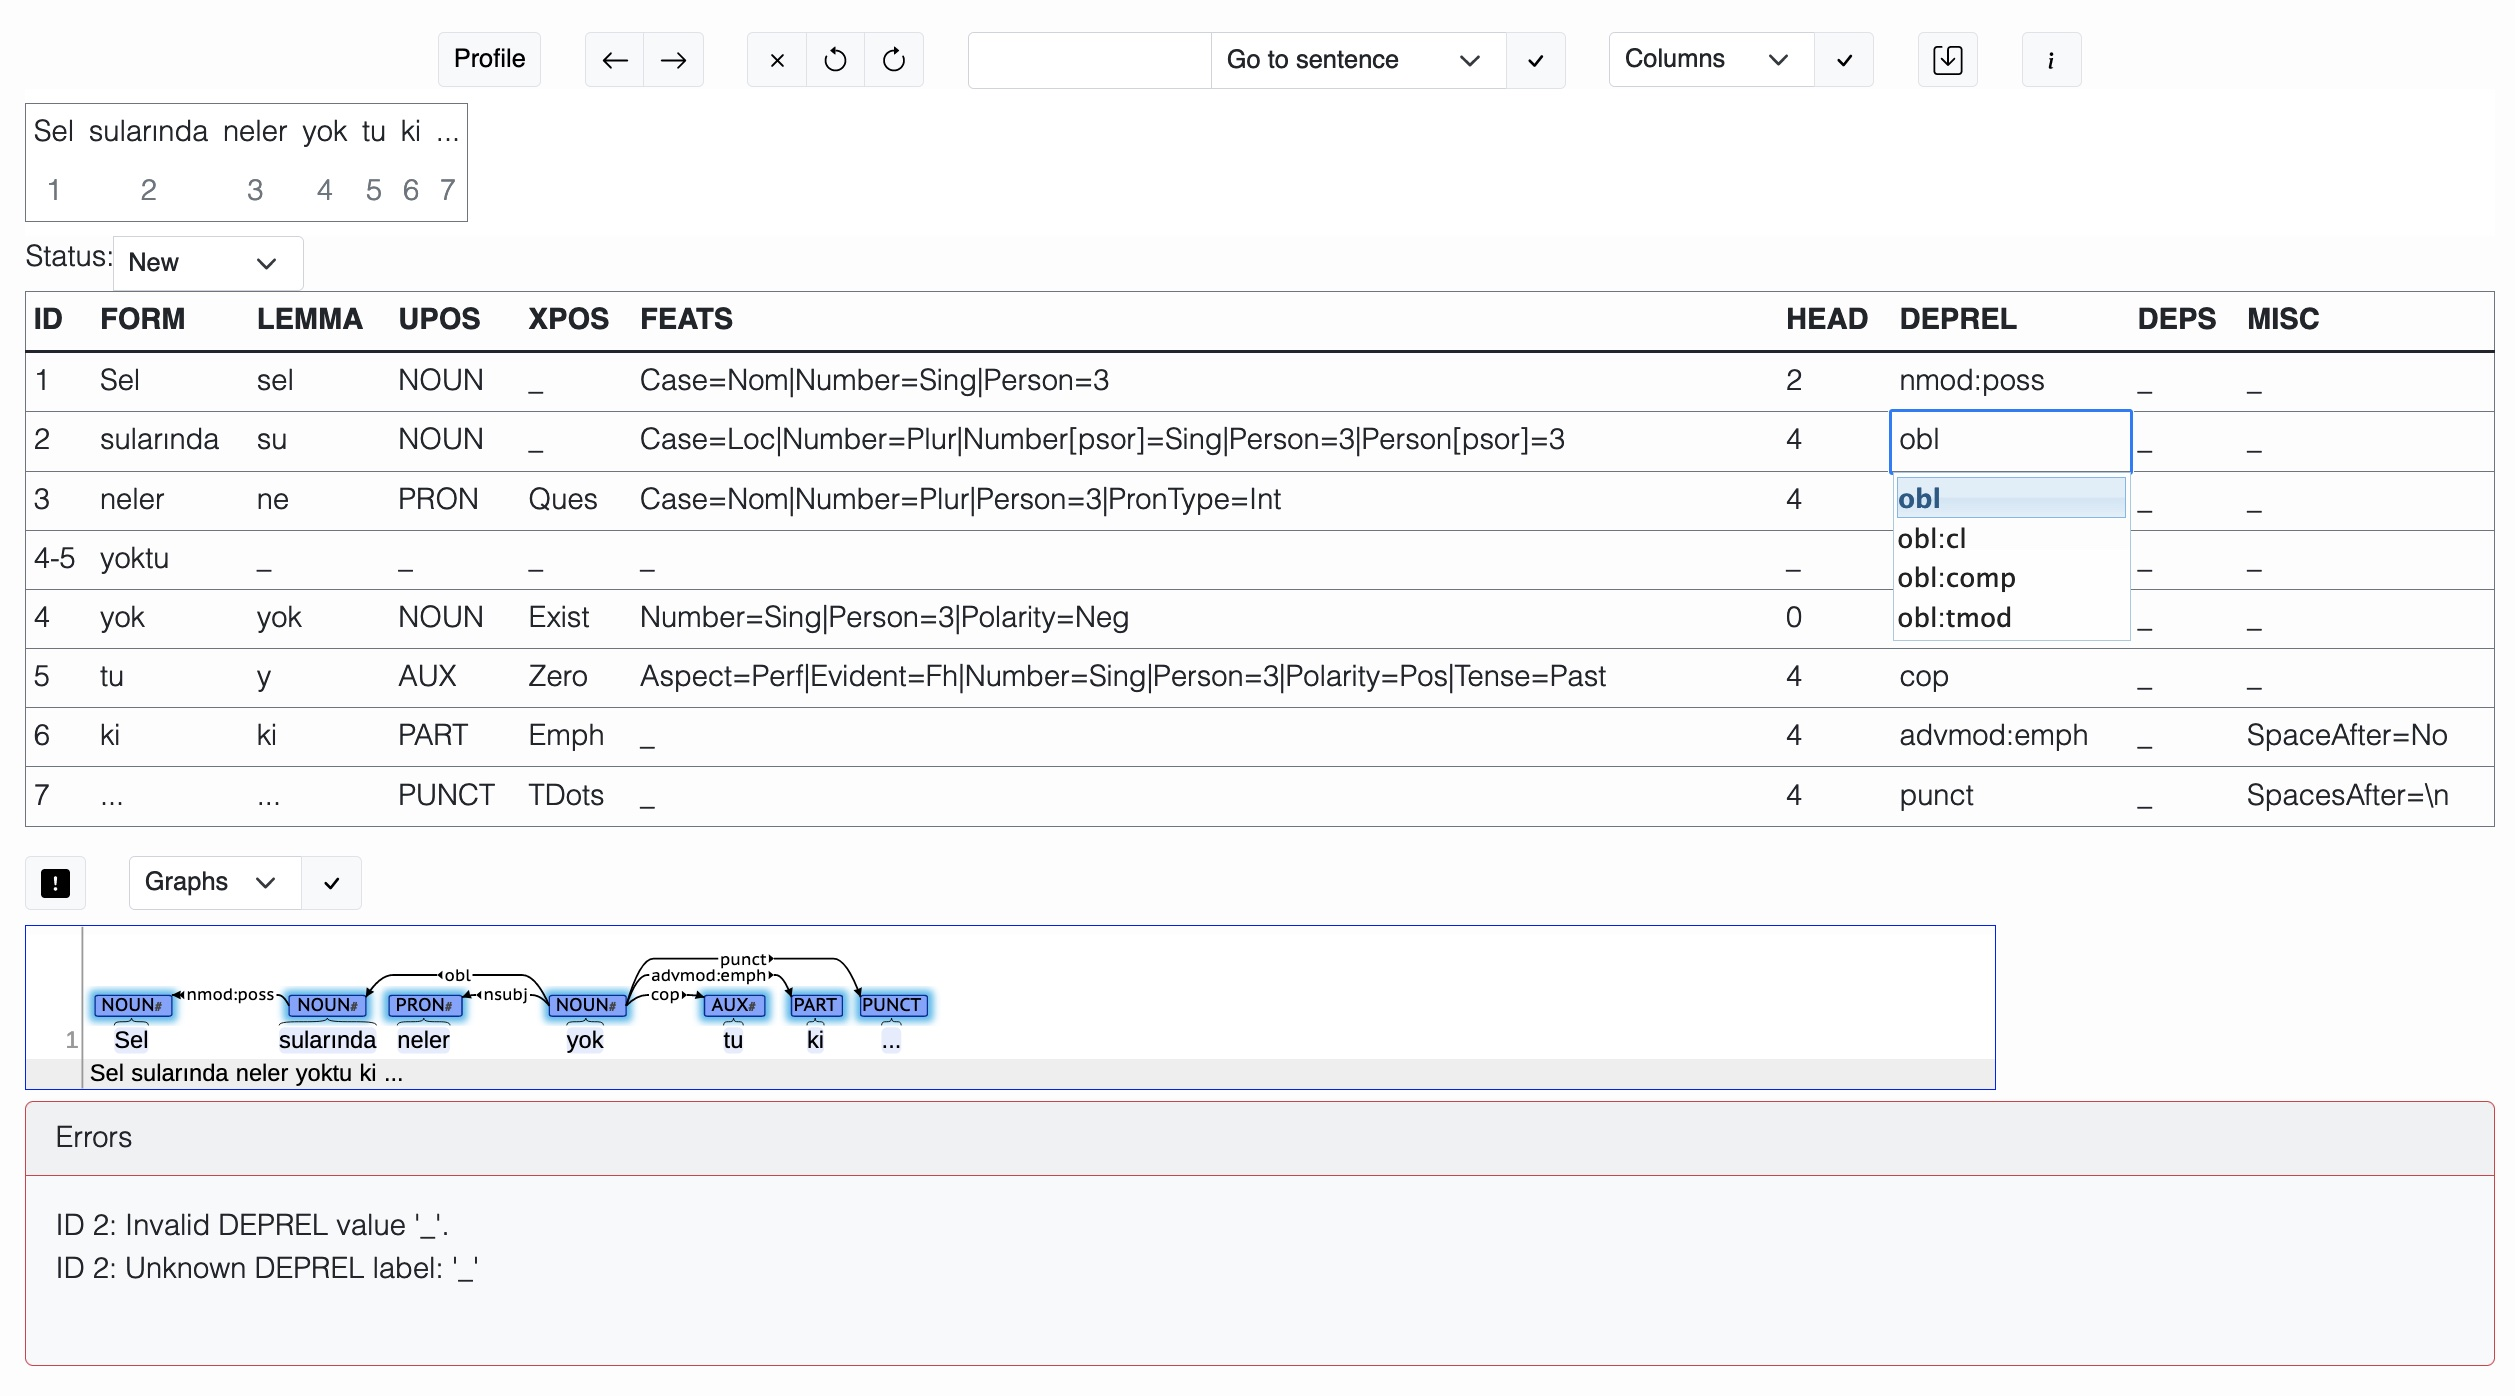
\includegraphics[width=0.8\textwidth]{boat-v2-sample-annotation-mac.jpg}}
    \caption{The annotation screen captured while the sentence ``Sel sularında neler yoktu ki...'' \textit{(‘What wasn't in the flood waters…’)} is being annotated. The \deprel\ tag for the surface form ``sularında'' is being annotated by selecting among the valid alternatives that appear in the pop-up. Selections can be made with the use of arrow keys.}
    \label{fig:anno-fig}
\end{figure}

A typical annotation can proceed as follows:
An annotator selects a sentence from a treebank.
An annotation table appears with the sentence parsed according to the \ud\ format.
Each row corresponds to a token and its annotations.
Figure~\ref{fig:anno-fig} shows the annotation view while an annotator is annotating a Turkish sentence ``Sel sularında neler yoktu ki...'' (translation: \textit{What wasn't in the flood waters...}).

An annotator can make use of dependency graphs, errors, and search during annotation.
Dependency graphs are visual cues for how lemmas are dependent upon one another.
Errors are helpful reminders compliant with \ud.
Searching can help the annotator disambiguate ambiguous forms, or check previously annotated sentences to ensure coherency and inter-annotator agreement.
The annotator can search for previously made annotations in combinations of text and feature values.

Annotators can customize the columns and dependency graph in accordance with their preferences.
They can hide and view columns as they prefer, and they can choose from several different dependency graph styles.
When an annotation is finished, its status can be set to ``Complete''.

% \section{Evaluation}
\label{sec:evaluation}

% earlier test ; may remove it?
Following the development phases of \boatvtwo, 4 test were conducted in order to evaluate the tool.
The aim of each test was to assess a different aspect of \boatvtwo.

\subsection{Version Comparison}
The first test was carried out in June 2022 to compare \boatvone\ and \boatvtwo.
As part of this test, two sets of 10 sentences were created.
Each set contained unique sentences with each sentence in the first set having another sentence with the same amount of tokens in the second set.
The reason behind this choice was to eliminate potential confounders so that the two versions of the tool could be compared in terms of annotator speed, responsiveness, and various other metrics.

A single annotator used \boatvone\ to annotate the first set, then used \boatvtwo to annotate the second set.
During both of the annotation processes, an observer took notes and timed how long it took to complete each sentence on each tool.
There was a noticeable speedup (approximately 30\%) using \boatvtwo.
Among the new features that were most appreciated are auto-completion, condensed dependency tree representation, a significant reduction in scrolling, keyword search, and searching by morphological features.
The non-search-related features proved to be instrumental in retaining focus.

\subsection{User Testing}
After version comparison, several test cases were carefully designed for user testing in July 2022.
These cases included testing various functionalities of the tool, such as creating annotator accounts, creating and uploading treebanks, annotating both simple\footnote{Simple sentence annotation refers to sentences with less than 10 tokens.} and complex sentences\footnote{Complex sentence annotation included long sentences which also required splitting lemmas.}, splitting and merging lemmas, changing preexisting annotation tags, viewing different dependency graphs, and searching in previously created annotations.

The goal of the test was to fully assess the responsiveness and functionality of \boatvtwo.
Thus, the cases covered both newly introduced functions like choosing different dependency graph styles and old functions like lemma splitting.
Three experienced linguist annotators carried out the user tests on different operating systems and browsers (Safari~\cite{safari} on macOS~\cite{macos}, Chrome~\cite{chrome} on Windows~\cite{windows}), all on desktop devices.
Following the tests, they filled out questionnaires to give feedback on whether they were able to carry out the annotations and operations they were expected to.
In addition, they reported any errors or issues they came across during the testing.
The test results were mostly matching what the expected results were.
The feedback provided by the participants was referred to while improving the tool further and making it more robust.

\subsection{Automated Testing}
After user testing, we wanted to construct automated testing scripts in order that the development does not produce unintended results, such as preventing a feature from working expectedly.
For this, we have designed and tested with several test cases via Selenium~\cite{selenium} in September 2022.
In these tests, we aimed to test if the tool's interface works as expected in various use cases, leveraging assertions in the tests.
These use cases included logging in, creating and deleting treebanks, and searching sentences.
The actual results of these tests were matching the expected results.
We plan to use these automated testing scripts when we update the corresponding web pages in these tests so that the development continues to improve the tool.

\subsection{Learnability and Intuitiveness}
The final round of testing targeted the learnability and intuitiveness of \boatvtwo.
For this purpose, a test case similar to the previous user testing was designed and carried out in December 2022.
This test case included numerous functionalities of the tool, such as creating and logging into a user account, creating and uploading a treebank, annotating parts of simple and complex sentences, changing preexisting annotations, merging lemmas, and searching in current and previously annotated treebanks.

% One undergraduate and one graduate students from the Department of Linguistics at Boğaziçi University  participated in this test.
Two linguists~\cite{anon} with no annotation experience participated in the test.
Before they started the test, they were introduced to the tool and the \ud\ framework by an experienced annotator for the first time.
They were shown how to use the tool and do annotations, and then they were given the dataset to be annotated.
They did the tests on the same device and browser they received the training on (Safari on a desktop macOS device).

As they carried out the tests, the participants were observed by the trainer who also took notes regarding the tests.
The participants were able to ask questions and get directions from the trainer regarding both the \ud\ framework and the annotation tool.
After testing, the participants were asked to fill out a questionnaire regarding their experience.
Their feedback and notes taken by the expert during the tests were considered together by the development team.
\section{Evaluation}
\label{sec:evaluation}

Following the development phases of \boatvtwo, 4 test were conducted in order to evaluate the tool.
The aim of each test was to assess a different aspect of \boatvtwo.

\subsection{Version Comparison}
The first test was carried out in June 2022 to compare \boatvone\ and \boatvtwo.
As part of this test, two sets of 10 sentences were created.
Each set contained unique sentences with each sentence in the first set having another sentence with the same amount of tokens in the second set.
The reason behind this choice was to eliminate potential confounders so that the two versions of the tool could be compared in terms of annotator speed, responsiveness, and various other metrics.

A single annotator used \boatvone\ to annotate the first set, then used \boatvtwo to annotate the second set.
During both of the annotation processes, an observer took notes and timed how long it took to complete each sentence on each tool.
There was a noticeable speedup (approximately 30\%) using \boatvtwo.
Among the new features that were most appreciated are auto-completion, condensed dependency tree representation, a significant reduction in scrolling, keyword search, and searching by morphological features.
The non-search-related features proved to be instrumental in retaining focus.

\subsection{User Testing}
After version comparison, several test cases were carefully designed for user testing in July 2022.
These cases included testing various functionalities of the tool, such as creating annotator accounts, creating and uploading treebanks, annotating both simple\footnote{Simple sentence annotation refers to sentences with less than 10 tokens.} and complex sentences\footnote{Complex sentence annotation included long sentences which also required splitting lemmas.}, splitting and merging lemmas, changing preexisting annotation tags, viewing different dependency graphs, and searching in previously created annotations.

The goal of the test was to fully assess the responsiveness and functionality of \boatvtwo.
Thus, the cases covered both newly introduced functions like choosing different dependency graph styles and old functions like lemma splitting.
Three experienced linguist annotators carried out the user tests on different operating systems and browsers (Safari~\cite{safari} on macOS~\cite{macos}, Chrome~\cite{chrome} on Windows~\cite{windows}), all on desktop devices.
Following the tests, they filled out questionnaires to give feedback on whether they were able to carry out the annotations and operations they were expected to.
In addition, they reported any errors or issues they came across during the testing.
The test results were mostly matching what the expected results were.
The feedback provided by the participants was referred to while improving the tool further and making it more robust.

\subsection{Automated Testing}
After user testing, we wanted to construct automated testing scripts in order that the development does not produce unintended results, such as preventing a feature from working expectedly.
For this, we have designed and tested with several test cases via Selenium~\cite{selenium} in September 2022.
In these tests, we aimed to test if the tool's interface works as expected in various use cases, leveraging assertions in the tests.
These use cases included logging in, creating and deleting treebanks, and searching sentences.
The actual results of these tests were matching the expected results.
We plan to use these automated testing scripts when we update the corresponding web pages in these tests so that the development continues to improve the tool.

\subsection{Learnability and Intuitiveness}
The final round of testing targeted the learnability and intuitiveness of \boatvtwo.
For this purpose, a test case similar to the previous user testing was designed and carried out in December 2022.
This test case included numerous functionalities of the tool, such as creating and logging into a user account, creating and uploading a treebank, annotating parts of simple and complex sentences, changing preexisting annotations, merging lemmas, and searching in current and previously annotated treebanks.

Two linguists~\cite{anon} with no annotation experience participated in the test.
Before they started the test, they were introduced to the tool and the \ud\ framework by an experienced annotator for the first time.
They were shown how to use the tool and do annotations, and then they were given the dataset to be annotated.
They did the tests on the same device and browser they received the training on (Safari on a desktop macOS device).

As they carried out the tests, the participants were observed by the trainer who also took notes regarding the tests.
The participants were able to ask questions and get directions from the trainer regarding both the \ud\ framework and the annotation tool.
After testing, the participants were asked to fill out a questionnaire regarding their experience.
Their feedback and notes taken by the expert during the tests were considered together by the development team.

% \section{Discussion and Conclusions}
\label{sec:discussion}

% subsections are needed ; for example, for testing
\todo[inline]{subsections are needed ; for example, for testing}

\boatvtwo\ aims to extend the functionality of \boatvone\ as a collaborative web-based application to support the annotation process based on previous experiences.
We developed a web application that supports agglutinative languages as described in Section~\ref{sec:implementation}.

The implementation choices served our goals well.
We believe that having experts in linguistics and experienced annotators in agglutinative treebank creation was instrumental in understanding the requirements and the design process.
We held numerous elicitation interviews and further meetings for clarifications and feedback requests.

We used modern software development tools and management practices during the development lifecycle of this tool.
The development of an API enables various extensions of this tool and access to the treebanks.
The containerization with Docker~\cite{docker} has facilitated easy delivery and deployment.
It is available on Boğaziçi University's NLP platform~\cite{TULAP} as an open-source resource.
The availability of the tool as a user as well as a developer is valuable for future use and developments.

% we've done some testing ; more testing and documentation here would be useful
This tool is in the testing phase and has had encouraging early feedback.
We compared the annotation of several sentences with the same number of tokens using \boatvone\ and \boatvtwo.
While we kept the number of words in a sentence constant, we did not use the same sentences since having previously annotated a sentence would impact the annotation on another version.
Keeping the number of words the same provides a somewhat comparable experience.
There was a noticeable speedup (approximately 30\%) using \boatvtwo.
% above testing need not be mentioned in this paper
Among the new features that are most appreciated are autocompletion, condensed dependency tree representation, significant reduction on scrolling, keyword search, and search by morphological features.
The non-search related features are instrumental to retaining focus.

We are encouraged by the early responses to this tool and anticipate its extensions.
In fact, our implementation of \boatvtwo\ resulted in a revision request for \boatvone\ to include the focus enhancing features.
This also resulted in significant speedup and improved user experience, which was reported as a qualitative observation by an annotator.
Presently, our testing is focused on more extensive cases (annotation of sentences with varying degrees of complexity) and, importantly, the multi-user functionalities.
For this purpose, we are in the process of recruiting several annotators with a background in linguistics.

\section{Discussion and Conclusions}
\label{sec:discussion}

Our aim with \boatvtwo\ is to develop a collaborative web-based application based on previous experiences, supporting the annotation process of many languages, specifically morphologically rich ones.
We believe that having experts in linguistics and annotators experienced in agglutinative treebank creation was instrumental in understanding the requirements and also in the design process.
We held numerous elicitation interviews and further meetings for clarifications.

We have used modern software development tools and management practices during the development lifecycle of this tool.
The API enables various extensions of the tool and also programmatic access to the treebanks.
The containerization with Docker~\cite{docker} eases the deployment procedure.
It is available~\cite{anon} as an open-source resource.
The wide availability of the tool is valuable for future use and developments.

We are encouraged by the evaluation performed on this tool and anticipate its extensions.
The feedback coming from the evaluation presents many ways that the tool can be improved.
For the tool's future, we plan on improving the current functionality, implementing annotation-centric new features, such as automated annotation of certain tags based on rules provided by annotators, or creating notes on annotations to communicate with other annotators through the application.
We also plan to implement support for various languages regarding auto-completion and annotation validation.

% 
\begin{thebibliography}{99}

\bibitem{anon} Anonymous. We're not including this reference to preserve anonymity for the review process.

\bibitem{altnlp} Akkurt SF, Marşan B, Uskudarli S. Boat v2 - A web-based dependency annotation tool with focus on agglutinative languages. In: Agglutinative Language Technologies as a challenge of Natural Language Processing (ALTNLP); Slovenia; 2022. https://doi.org/10.48550/arXiv.2207.01327

\bibitem{brat} Stenetorp P, Pyysalo S, Topi\'{c} G, Ohta T, Ananiadou S et al. brat: a web-based tool for nlp-assisted text annotation. In: Proceedings of the Demonstrations Session at EACL; Avignon, France; 2012. Association for Computational Linguistics.

\bibitem{conll-u_editor} Heinecke J. Conllueditor: a fully graphical editor for universal dependencies treebank files. In: Universal Dependencies Workshop; Paris; 2019.

\bibitem{itu-annotation-tool} Pamay T, Sulubacak U, Toruno{\u{g}}lu-Selamet D, Eryi{\u{g}}it G. The annotation process of the itu web treebank. In: Proceedings of The 9th Linguistic Annotation Workshop; Denver, Colorado, USA; 2015. Association for Computational Linguistics, pp. 95-101. https://doi.org/10.3115/v1/W15-1610

\bibitem{conll} Buchholz S, Marsi E. Conll-x shared task on multilingual dependency parsing. In: Proceedings of the Tenth Conference on Computational Natural Language Learning (CoNLL-X); New York City; 2006. Association for Computational Linguistics, pp. 149-164.

\bibitem{stardust} Yenice AB, Cesur N, Kuzgun A, Y{\i}ld{\i}z OT. Introducing stardust: a ud-based dependency annotation tool. In: Proceedings of the 16th Linguistic Annotation Workshop (LAW-XVI) within LREC2022; Marseille, France; 2022. European Language Resources Association; pp. 79-84.

\bibitem{ud-annotatrix} Francis MT, Mariya S, Jonathan NW. Ud annotatrix: an annotation tool for universal dependencies. In: Proceedings of the 16th International Workshop on Treebanks and Linguistic Theories (TLT16); 2018; pp. 10-17.

\bibitem{bootstrap} Bootstrap (2022). Bootstrap [online]. Website https://getbootstrap.com/docs/5.1 [accessed 05 May 2022].

\bibitem{cg3} Didriksen T (2022). Constraint Grammar Manual [online]. Website https://visl.sdu.dk/cg3/single/ [accessed 18 November 2022].

\bibitem{dgannotator} Attardi G (2022). {DgAnnotator} [online]. Website http://medialab.di.unipi.it/Project/QA/Parser/DgAnnotator/ [accessed 27 March 2022].

\bibitem{django} Django Software Foundation (2022). Django documentation [online]. Website https://docs.djangoproject.com/en/4.0 [accessed 25 March 2022].

\bibitem{django-filter} Alex Gaynor, Carlton Gibson and others (2022). django-filter [online]. Website https://docs.djangoproject.com/en/4.0 [accessed 24 April 2022].

\bibitem{docker} Docker Inc. (2022). Docker [online]. Website https://www.docker.com [accessed 2 May 2022].

\bibitem{drf} Encode OSS Ltd. (2022). Django REST framework [online]. Website https://www.django-rest-framework.org [accessed 27 March 2022].

\bibitem{dropbox} Dropbox, Inc. (2022). Dropbox.com [online]. Website http://dropbox.com [accessed 18 November 2022].

\bibitem{psql} The PostgreSQL Global Development Group (2022). PostgreSQL [online]. Website https://www.postgresql.org/docs [accessed 27 March 2022].

\bibitem{mysql} Oracle (2022). MySQL [online]. Website https://www.mysql.com/ [accessed 16 December 2022].

\bibitem{tomcat} The Apache Software Foundation (2022). Apache Tomcat® [online]. Website https://tomcat.apache.org/ [accessed 16 December 2022].

\bibitem{java} Oracle (2022). Oracle Java Technologies [online]. Website https://www.oracle.com/java/technologies/ [accessed 16 December 2022].

\bibitem{python} Python Software Foundation (2022). Python [online]. Website https://www.python.org [accessed 24 April 2022].

\bibitem{qt} The Qt Company (2022). Qt [online]. Website https://www.qt.io/ [accessed 25 May 2022].

\bibitem{spacy} Explosion (2022). spaCy [online]. Website https://spacy.io [accessed 27 March 2022].

\bibitem{spyssalo} Pyysalo S (2022). conllu.js [online]. Website http://spyysalo.github.io/conllu.js [accessed 25 March 2022].

\bibitem{ud} Universal Dependencies (2022). UD [online]. Website https://universaldependencies.org [accessed 2 May 2022].

\bibitem{ud-tools} Universal Dependencies (2022). UD tools [online]. Website https://universaldependencies.org/tools [accessed 22 April 2022].

\bibitem{webanno} WebAnno (2022). WebAnno [online]. Website https://webanno.github.io/webanno/documentation [accessed 5 May 2022].

\bibitem{atis-en} Universal Dependencies (2021). UD English Atis [online]. Website https://universaldependencies.org/treebanks/en\_atis/index.html [accessed 4 Jan 2023].

\bibitem{atis-tr} Universal Dependencies (2021). UD Turkish Atis [online]. Website https://universaldependencies.org/treebanks/tr\_atis/index.html [accessed 4 Jan 2023].

\bibitem{pud-en} Universal Dependencies (2021). UD English PUD [online]. Website https://universaldependencies.org/treebanks/en\_pud/index.html [accessed 4 Jan 2023].

\bibitem{pud-tr} Universal Dependencies (2021). UD Turkish PUD [online]. Website https://universaldependencies.org/treebanks/tr\_pud/index.html [accessed 4 Jan 2023].

\bibitem{macos} Apple Inc. (2022). macOS [online]. Website https://www.apple.com/macos/ [accessed 5 Jan 2023].

\bibitem{safari} Apple Inc. (2022). Safari [online]. Website https://www.apple.com/safari/ [accessed 5 Jan 2023].

\bibitem{windows} Microsoft (2022). Windows [online]. Website https://www.microsoft.com/en-us/windows [accessed 5 Jan 2023].

\bibitem{chrome} Google (2022). Google Chrome [online]. Website https://www.google.com/chrome/ [accessed 5 Jan 2023].

\bibitem{selenium} Selenium (2022). Software Freedom Conservancy [online]. Website https://www.selenium.dev/ [accessed 5 Jan 2023].

\end{thebibliography}

\begin{thebibliography}{99}

\bibitem{anon} Anonymous. We're not including this reference to preserve anonymity for the review process.

\bibitem{brat} Stenetorp P, Pyysalo S, Topi\'{c} G, Ohta T, Ananiadou S et al. brat: a web-based tool for nlp-assisted text annotation. In: Proceedings of the Demonstrations Session at EACL; Avignon, France; 2012. Association for Computational Linguistics.

\bibitem{conll-u_editor} Heinecke J. Conllueditor: a fully graphical editor for universal dependencies treebank files. In: Universal Dependencies Workshop; Paris; 2019.

\bibitem{itu-annotation-tool} Pamay T, Sulubacak U, Toruno{\u{g}}lu-Selamet D, Eryi{\u{g}}it G. The annotation process of the itu web treebank. In: Proceedings of The 9th Linguistic Annotation Workshop; Denver, Colorado, USA; 2015. Association for Computational Linguistics, pp. 95-101. https://doi.org/10.3115/v1/W15-1610

\bibitem{conll} Buchholz S, Marsi E. Conll-x shared task on multilingual dependency parsing. In: Proceedings of the Tenth Conference on Computational Natural Language Learning (CoNLL-X); New York City; 2006. Association for Computational Linguistics, pp. 149-164.

\bibitem{stardust} Yenice AB, Cesur N, Kuzgun A, Y{\i}ld{\i}z OT. Introducing stardust: a ud-based dependency annotation tool. In: Proceedings of the 16th Linguistic Annotation Workshop (LAW-XVI) within LREC2022; Marseille, France; 2022. European Language Resources Association; pp. 79-84.

\bibitem{ud-annotatrix} Francis MT, Mariya S, Jonathan NW. Ud annotatrix: an annotation tool for universal dependencies. In: Proceedings of the 16th International Workshop on Treebanks and Linguistic Theories (TLT16); 2018; pp. 10-17.

\bibitem{bootstrap} Bootstrap (2022). Bootstrap [online]. Website https://getbootstrap.com/docs/5.1 [accessed 05 May 2022].

\bibitem{cg3} Didriksen T (2022). Constraint Grammar Manual [online]. Website https://visl.sdu.dk/cg3/single/ [accessed 18 November 2022].

\bibitem{dgannotator} Attardi G (2022). {DgAnnotator} [online]. Website http://medialab.di.unipi.it/Project/QA/Parser/DgAnnotator/ [accessed 27 March 2022].

\bibitem{django} Django Software Foundation (2022). Django documentation [online]. Website https://docs.djangoproject.com/en/4.0 [accessed 25 March 2022].

\bibitem{django-filter} Alex Gaynor, Carlton Gibson and others (2022). django-filter [online]. Website https://docs.djangoproject.com/en/4.0 [accessed 24 April 2022].

\bibitem{docker} Docker Inc. (2022). Docker [online]. Website https://www.docker.com [accessed 2 May 2022].

\bibitem{drf} Encode OSS Ltd. (2022). Django REST framework [online]. Website https://www.django-rest-framework.org [accessed 27 March 2022].

\bibitem{dropbox} Dropbox, Inc. (2022). Dropbox.com [online]. Website http://dropbox.com [accessed 18 November 2022].

\bibitem{psql} The PostgreSQL Global Development Group (2022). PostgreSQL [online]. Website https://www.postgresql.org/docs [accessed 27 March 2022].

\bibitem{mysql} Oracle (2022). MySQL [online]. Website https://www.mysql.com/ [accessed 16 December 2022].

\bibitem{tomcat} The Apache Software Foundation (2022). Apache Tomcat® [online]. Website https://tomcat.apache.org/ [accessed 16 December 2022].

\bibitem{java} Oracle (2022). Oracle Java Technologies [online]. Website https://www.oracle.com/java/technologies/ [accessed 16 December 2022].

\bibitem{python} Python Software Foundation (2022). Python [online]. Website https://www.python.org [accessed 24 April 2022].

\bibitem{qt} The Qt Company (2022). Qt [online]. Website https://www.qt.io/ [accessed 25 May 2022].

\bibitem{spacy} Explosion (2022). spaCy [online]. Website https://spacy.io [accessed 27 March 2022].

\bibitem{spyssalo} Pyysalo S (2022). conllu.js [online]. Website http://spyysalo.github.io/conllu.js [accessed 25 March 2022].

\bibitem{ud} Universal Dependencies (2022). UD [online]. Website https://universaldependencies.org [accessed 2 May 2022].

\bibitem{ud-tools} Universal Dependencies (2022). UD tools [online]. Website https://universaldependencies.org/tools [accessed 22 April 2022].

\bibitem{webanno} WebAnno (2022). WebAnno [online]. Website https://webanno.github.io/webanno/documentation [accessed 5 May 2022].

\bibitem{atis-en} Universal Dependencies (2021). UD English Atis [online]. Website https://universaldependencies.org/treebanks/en\_atis/index.html [accessed 4 Jan 2023].

\bibitem{atis-tr} Universal Dependencies (2021). UD Turkish Atis [online]. Website https://universaldependencies.org/treebanks/tr\_atis/index.html [accessed 4 Jan 2023].

\bibitem{pud-en} Universal Dependencies (2021). UD English PUD [online]. Website https://universaldependencies.org/treebanks/en\_pud/index.html [accessed 4 Jan 2023].

\bibitem{pud-tr} Universal Dependencies (2021). UD Turkish PUD [online]. Website https://universaldependencies.org/treebanks/tr\_pud/index.html [accessed 4 Jan 2023].

\bibitem{macos} Apple Inc. (2022). macOS [online]. Website https://www.apple.com/macos/ [accessed 5 Jan 2023].

\bibitem{safari} Apple Inc. (2022). Safari [online]. Website https://www.apple.com/safari/ [accessed 5 Jan 2023].

\bibitem{windows} Microsoft (2022). Windows [online]. Website https://www.microsoft.com/en-us/windows [accessed 5 Jan 2023].

\bibitem{chrome} Google (2022). Google Chrome [online]. Website https://www.google.com/chrome/ [accessed 5 Jan 2023].

\bibitem{selenium} Selenium (2022). Software Freedom Conservancy [online]. Website https://www.selenium.dev/ [accessed 5 Jan 2023].

\end{thebibliography}

\end{document}
